\documentclass[11pt]{article}

% DOCUMENT
\usepackage[english]{babel}
\usepackage[utf8]{inputenc}
\usepackage{setspace}
\usepackage[top=0.80in, bottom=0.80in, left=0.75in, right=0.75in]{geometry}
\usepackage{cmap}
\usepackage[T1]{fontenc}
%\usepackage[document]{ragged2e}
\usepackage[colorinlistoftodos]{todonotes}
\usepackage[colorlinks=true, allcolors=blue]{hyperref}
\usepackage{ragged2e} 
\usepackage{booktabs}
\usepackage[font=footnotesize,skip=1pt]{caption}
\newcommand{\source}[1]{\caption*{Source: {#1}} }
%\captionsetup{font=footnotesize}
\onehalfspacing
\usepackage{titling}
\usepackage{sectsty}
\usepackage{float}
\usepackage{comment}

% MATH
\usepackage{amsmath}
\usepackage{mathtools,amssymb}
\usepackage{amstext}
\usepackage{amsfonts}

% GRAPHICS
\usepackage{graphicx}
\usepackage{epstopdf}
\usepackage{adjustbox}
\usepackage{subcaption}


\usepackage{subcaption,rotating,natbib}
\usepackage{indentfirst}
\usepackage{natbib}
%\usepackage[font={small}]{caption}
%\usepackage[font={footnotesize}]{subcaption}
\usepackage{adjustbox}
\usepackage{amssymb}
\usepackage{bm}
%\usepackage[table]{xcolor}
\usepackage{tabu}
\usepackage{makecell}
\usepackage{longtable}
\usepackage{multirow}
\usepackage[normalem]{ulem}
\usepackage{etoolbox}
\usepackage{tabularx}
\usepackage{threeparttablex}
\usepackage[capposition=top]{floatrow}
%\usepackage{subcaption}
\usepackage{pdfpages}
\usepackage{pdflscape}
\usepackage{natbib}
\usepackage{enumitem}
\usepackage{pdfpages}

\newcommand{\partt}[2]{\frac{\partial #1}{\partial #2}} %the [2] indicates there will be 2 elements. This command defines a partial derivative where 2 arguments are numerator and denominator.

%% When I use \subsection{} "Tema XX:" shows up
%\renewcommand{\thesubsection}{Tema \arabic{subsection}:}
\renewcommand{\thesubsection}{Tema \thechapter\number\numexpr\value{subsection}-1\relax:}

%Command for text after subtitles to start in the same line
\usepackage{titlesec} 
\titleformat{\subsection}[runin]
  {\normalfont\large\bfseries}{\thesubsection}{1em}{}

\input{glyphtounicode}
\pdfgentounicode=1
\usepackage[none]{hyphenat}

\usepackage[at]{easylist}

%\title{ \LARGE Herramientas Computacionales de Investigación \\
%Trabajo Práctico 2: QGIS}
%\author{Felipe García Vassallo \\
%Rocío Senra}
%\date{}


\begin{document}

\begin{titlepage} % Suppresses displaying the page number on the title page and the subsequent page counts as page 1
	\newcommand{\HRule}{\rule{\linewidth}{0.5mm}} % Defines a new command for horizontal lines, change thickness here
	
	\center % Centre everything on the page
	
	%------------------------------------------------
	%	Headings
	%------------------------------------------------
	
\includegraphics[width=0.7\textwidth]{Airbnb/logoudesa}\\[0.8cm]
	\textsc{\LARGE Herramientas Computacionales de Investigación}\\[0.5cm] % Major heading such as course name
	
	\textsc{\Large María Amelia Gibbons}\\
	\vspace{4pt}
	%------------------------------------------------
	%	Title
	%------------------------------------------------
	\textcolor{white}{\HRule}\\[0.6cm]
	\huge\bfseries Trabajo Práctico 2: QGIS 
	\textcolor{white}{\HRule}\\[1.5cm]
	%------------------------------------------------
	%	Author(s)
	%------------------------------------------------
	\begin{center}
		\Large
		\textsc{Felipe García Vassallo\\
		        Rocío Senra}\\
	\end{center}
	
	% If you don't want a supervisor, uncomment the two lines below and comment the code above
	%{\large\textit{Author}}\\
	%John \textsc{Smith} % Your name
	
	%------------------------------------------------
	%	Date
	%------------------------------------------------
	\vfill\vfill\vfill % Position the date 3/4 down the remaining page
	{\large 2022}
	\vfill
	
\end{titlepage}

\section*{Ejercicio 1: Airbnb} 
%Crear 3 mapas y 3 gráficos a partir de los datos de Airbnb, describir qué tipo de mapa es, por qué eligieron hacer ese mapa/gráfico y qué muestra. 

\textbf{Mapa 1}
El siguiente mapa es un cartograma, donde se muestra la cantidad de crímenes cada 100 habitantes por \textit{community} en la ciudad de Chicago. La escala de colores indica cuáles son las zonas con mayor cantidad de crímenes cada 100 habitantes: el color más claro indica una menor cantidad de crímenes, mientras que el más oscuro una mayor cantidad. Asimismo, este tipo de mapa ajusta el tamaño de cada \textit{community} de acuerdo a la cantidad de crímenes que reporta.

\begin{figure}[H]
    \centering
    \caption{Cartograma sobre crímenes en Chicago}
	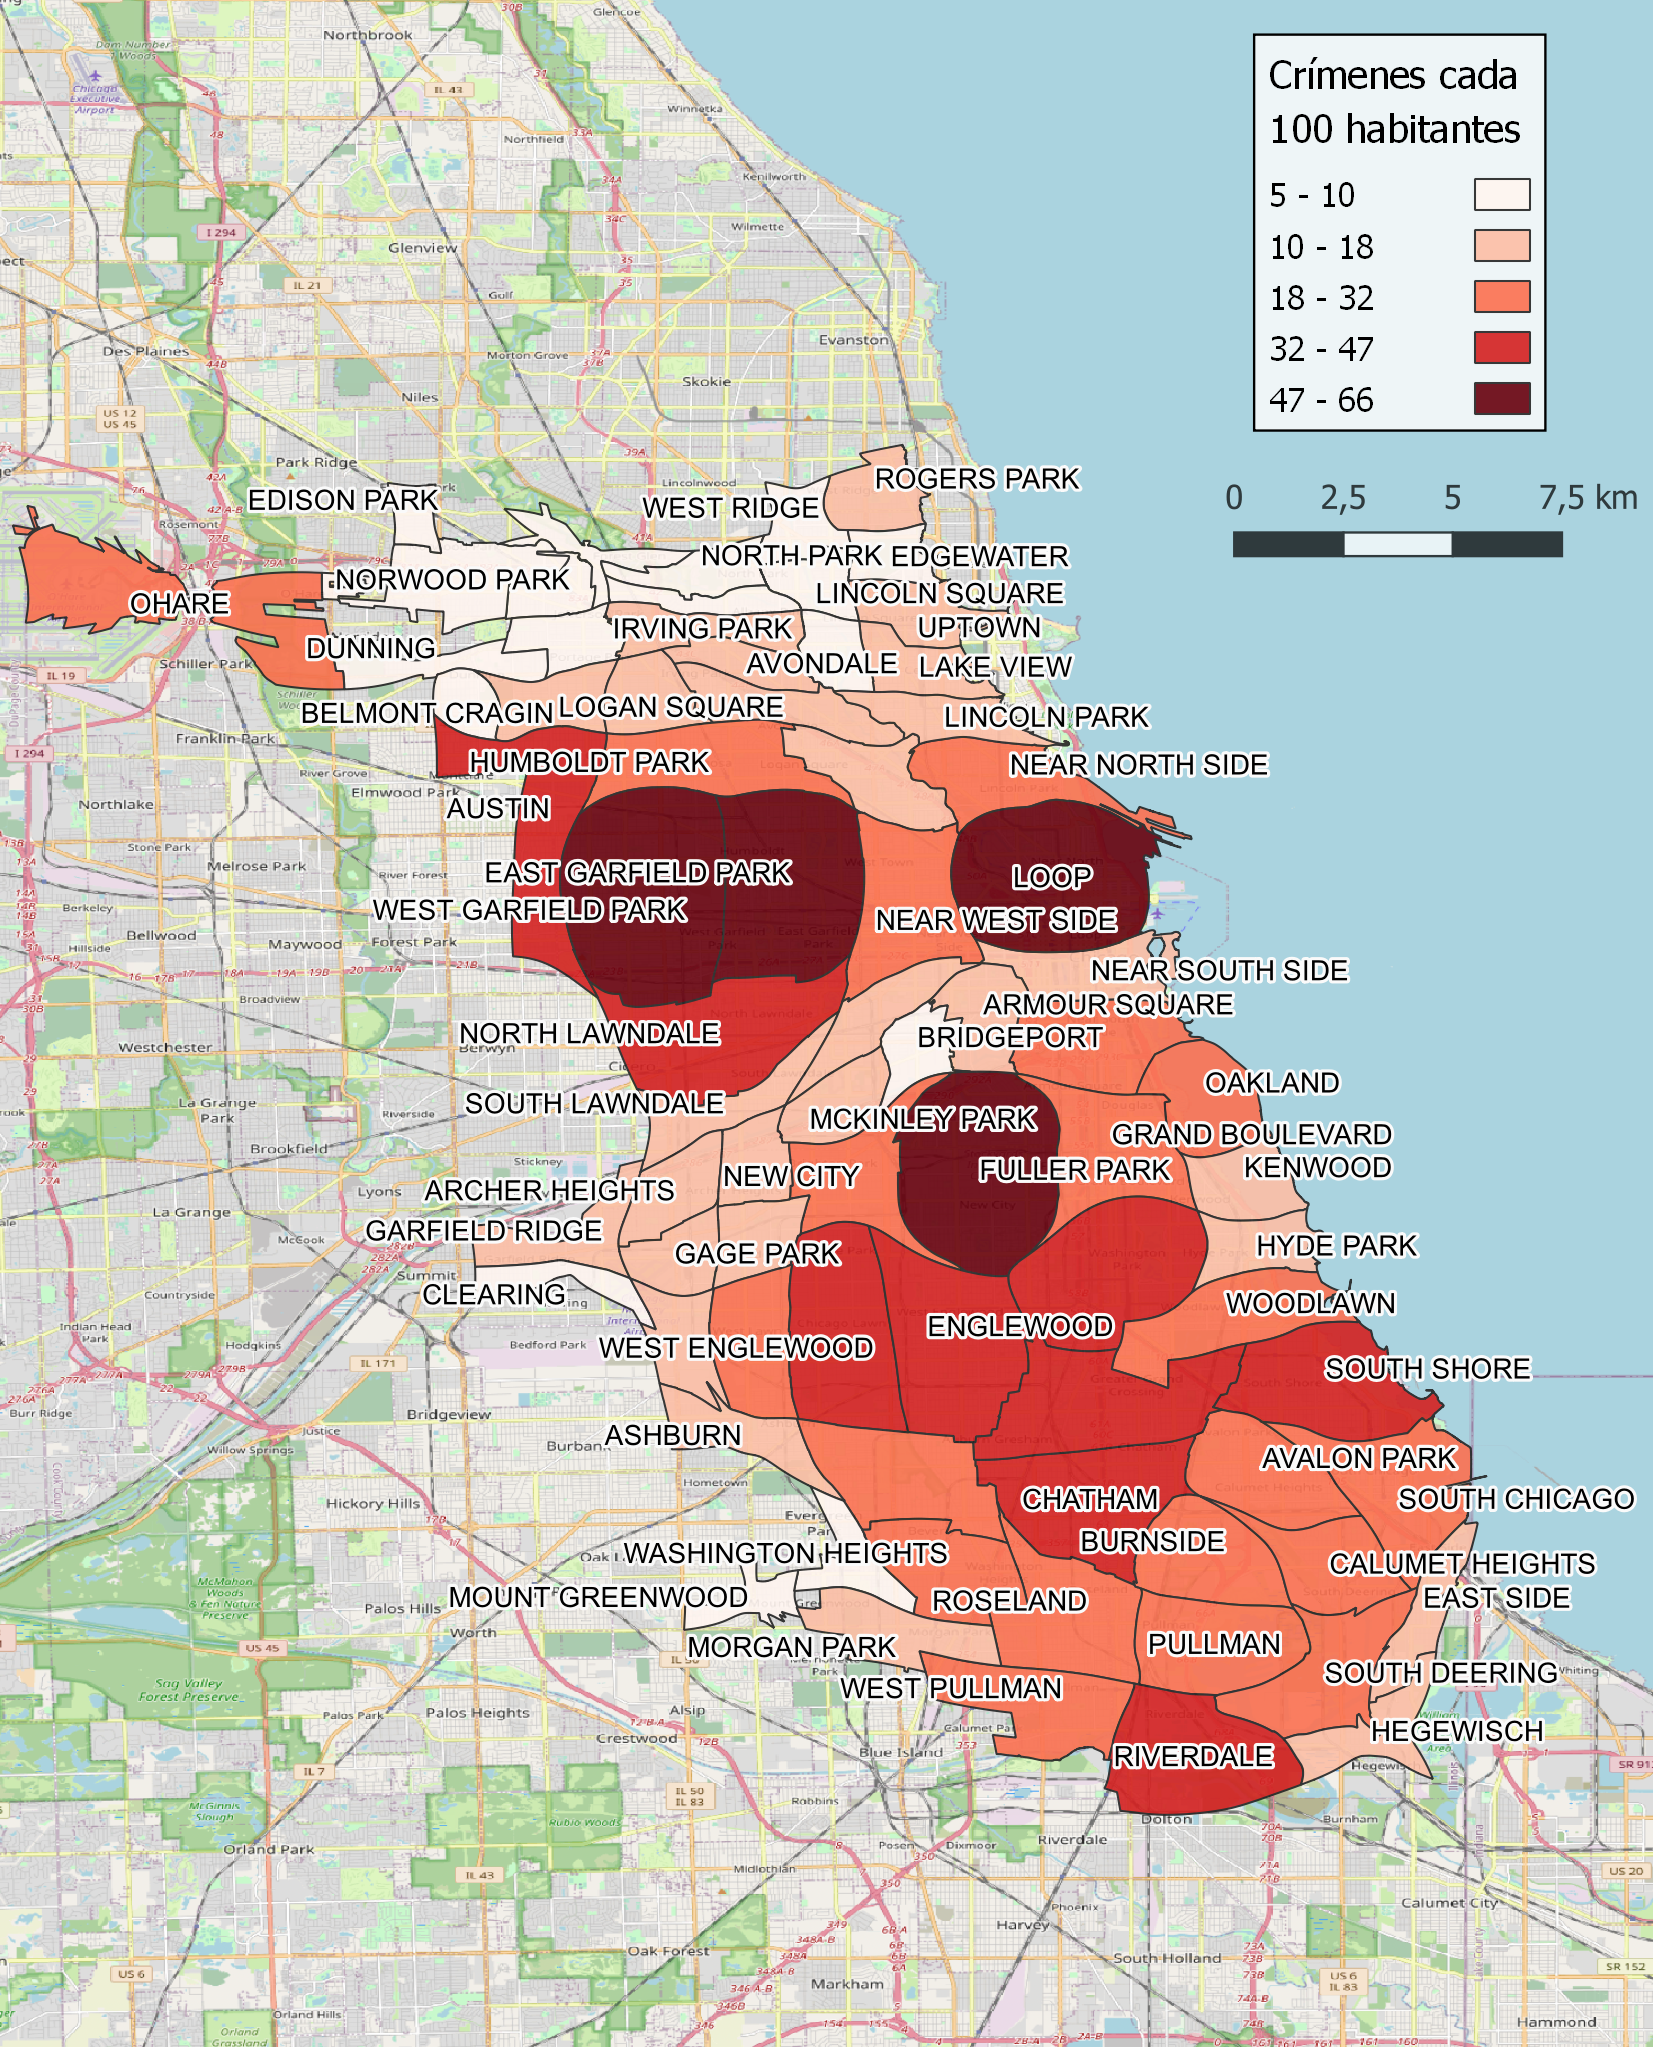
\includegraphics[scale=0.6]{Airbnb/Gráficos/mapa 1 airbnb}    
    \source{Chicago Data Portal.}
    \label{fig:carto}
\end{figure}

\newpage
\textbf{Mapa 2} En el mapa a continuación se muestra la distribución del ingreso per cápita en Chicago. En particular, se construyeron 6 categorías de ingreso per cápita, siendo la categoría 1 la de menor ingreso per cápita y la 6 la de mayor ingreso. A partir del mapa, se observa que la región suroeste de Chicago es la de menor ingreso per cápita.


\begin{figure}[H]
    \centering
    \caption{Ingreso per cápita}
    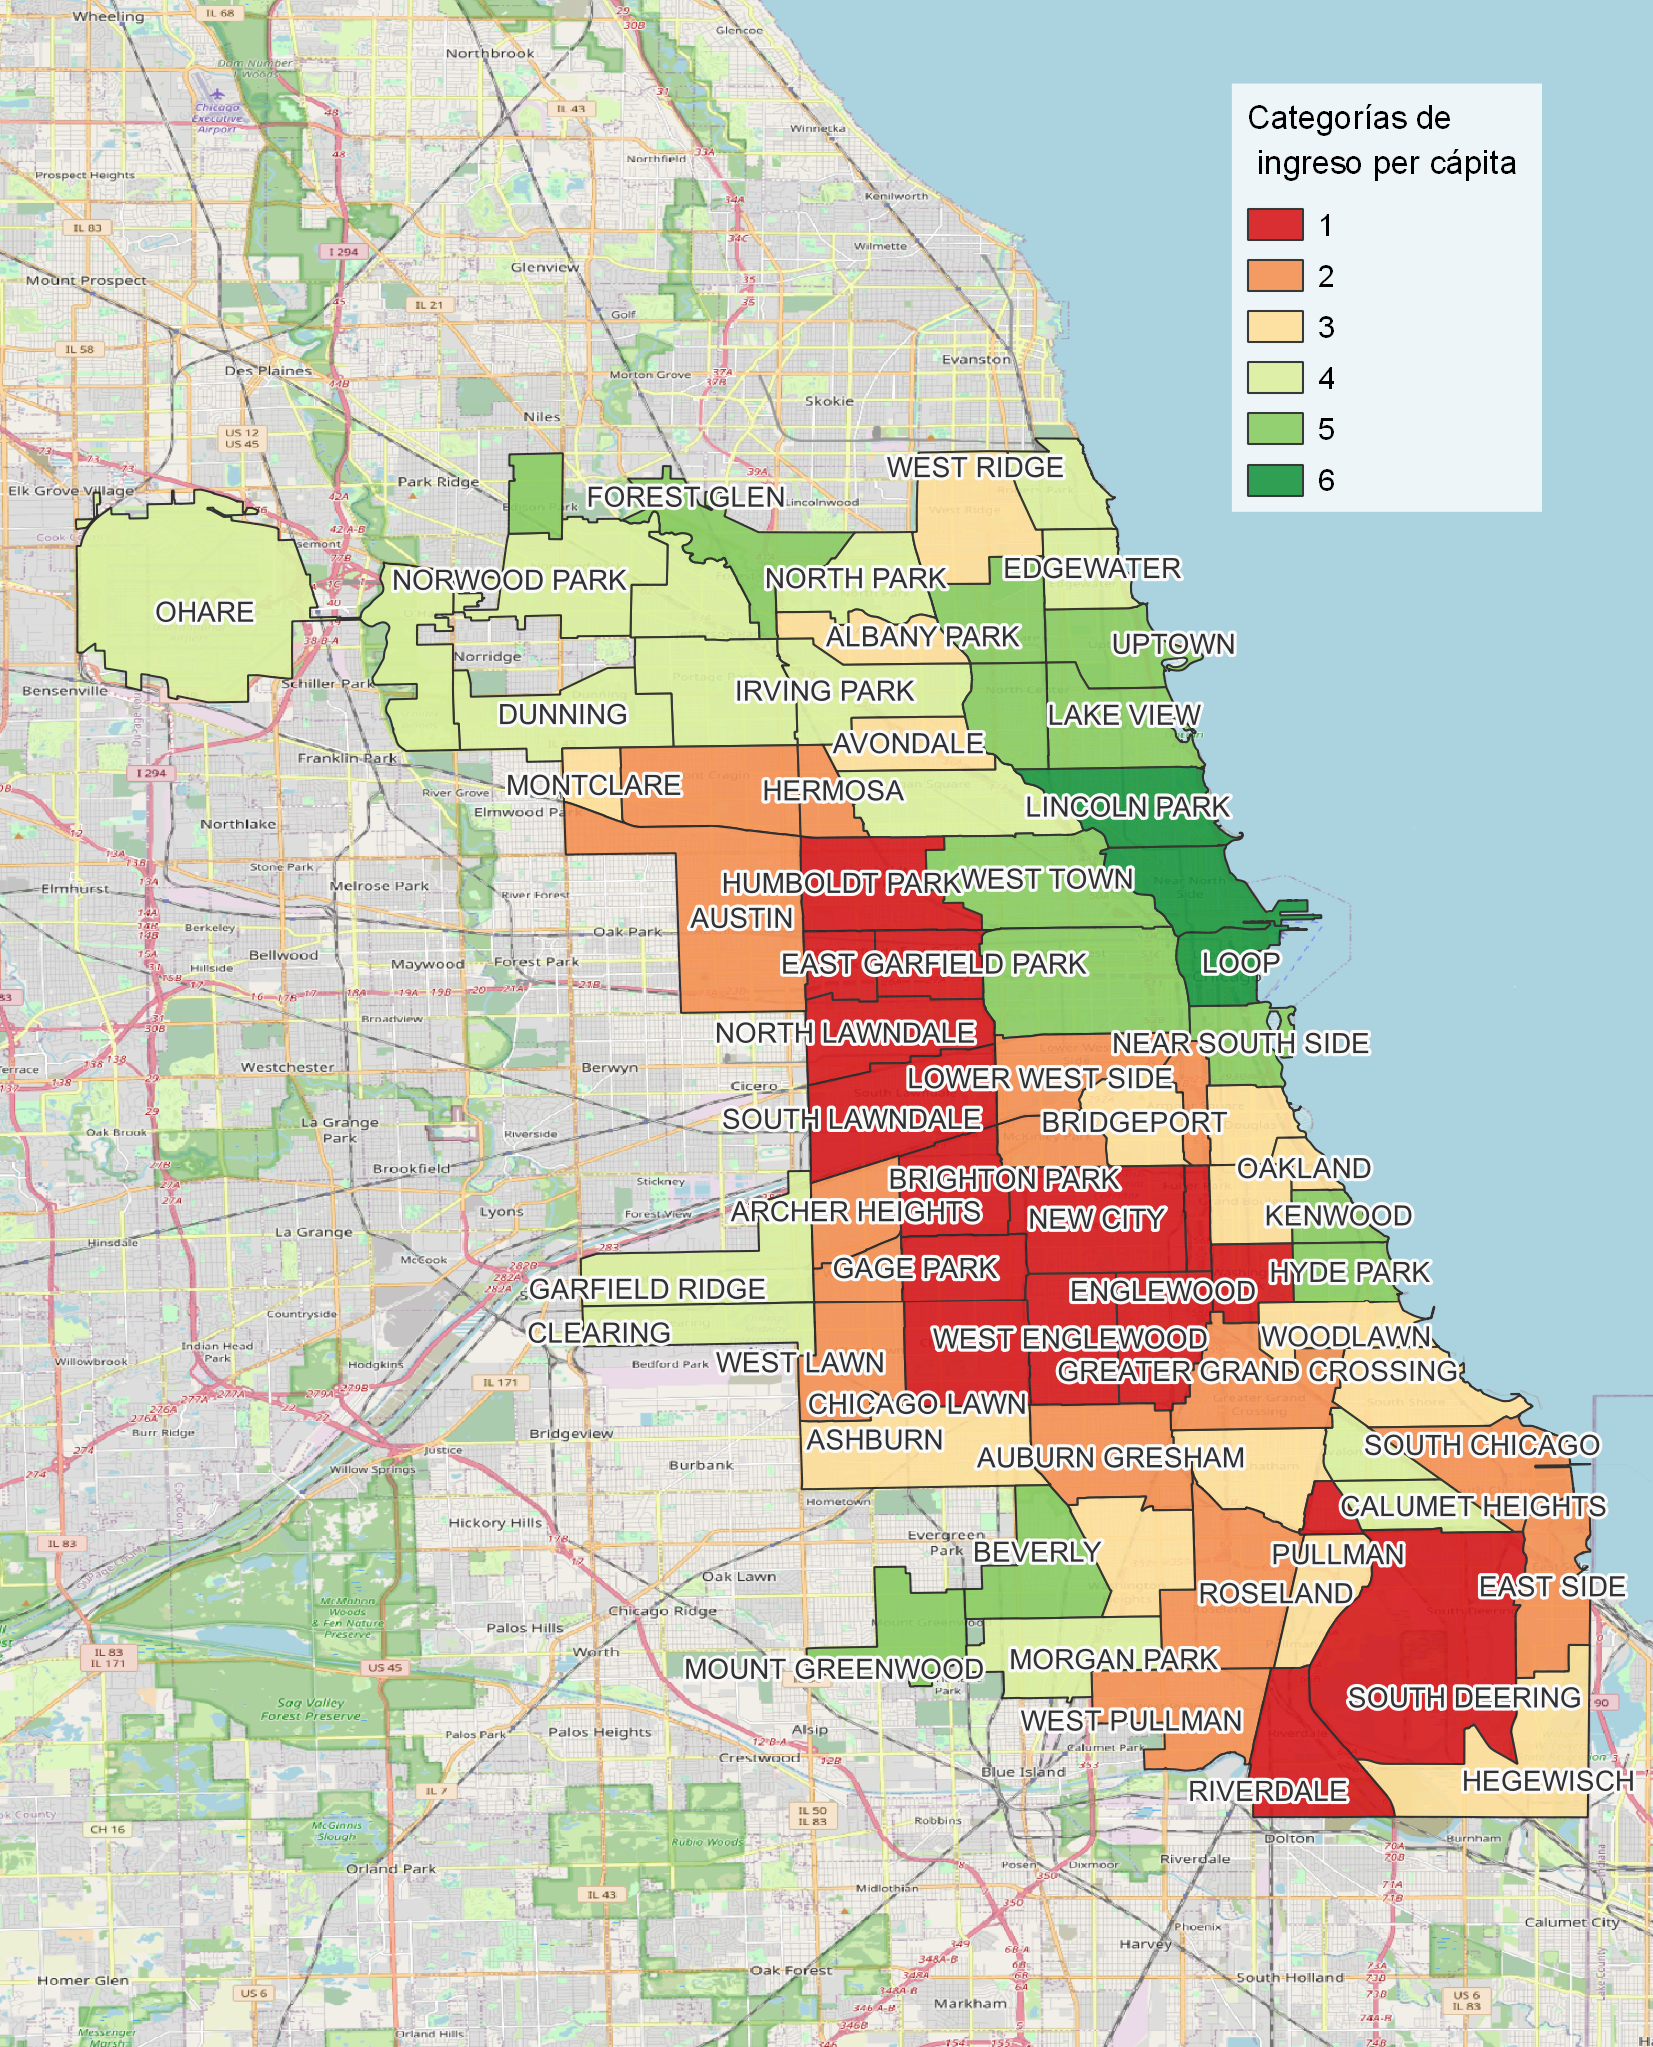
\includegraphics[scale=0.6]{Airbnb/Gráficos/mapa 2 airbnb.png}
    \source{Chicago Data Portal.}
    \label{fig:i_pc}
\end{figure}


\newpage
\textbf{Mapa 3} En el siguiente mapa se muestra, por un lado, el porcentaje de hogares sobrepoblados en Chicago y, por otro lado, la cantidad de unidades ofrecidas en Airbnb. Como sería esperable, la mayor parte de la oferta de Airbnb (en azul) se ubica alrededor del centro de la ciudad y en la zona norte de la misma, mientras que la mayoría de los hogares con sobrepoblación se ubican en las afueras de la ciudad. Asimismo, en relación al Mapa 2, se observa que la región con mayor sobrepoblación coincide en gran medida con la región de menor ingreso per cápita. 


\begin{figure}[H]
    \centering
    \caption{Sobrepoblación y oferta Airbnb}
    \includegraphics[scale=0.6]{Airbnb/Gráficos/mapa 3 airbnb.png}
    \source{Chicago Data Portal y Inside Airbnb.}
    \label{fig:crowd_air}
\end{figure}

\newpage

\textbf{Gráfico 1} Este es un \textit{scatter plot} que muestra la relación entre la proporción de hogares bajo la línea de pobreza y cantidad de crímenes cada 100 habitantes todas las comunidades de Chicago. Elegimos este tipo de gráfico para ver la correlación entre estas dos variables. La figura muestra una relación lineal positiva entre crimen y pobreza.

\begin{figure}[H]
    \centering
    \caption{Pobreza y crimen}
    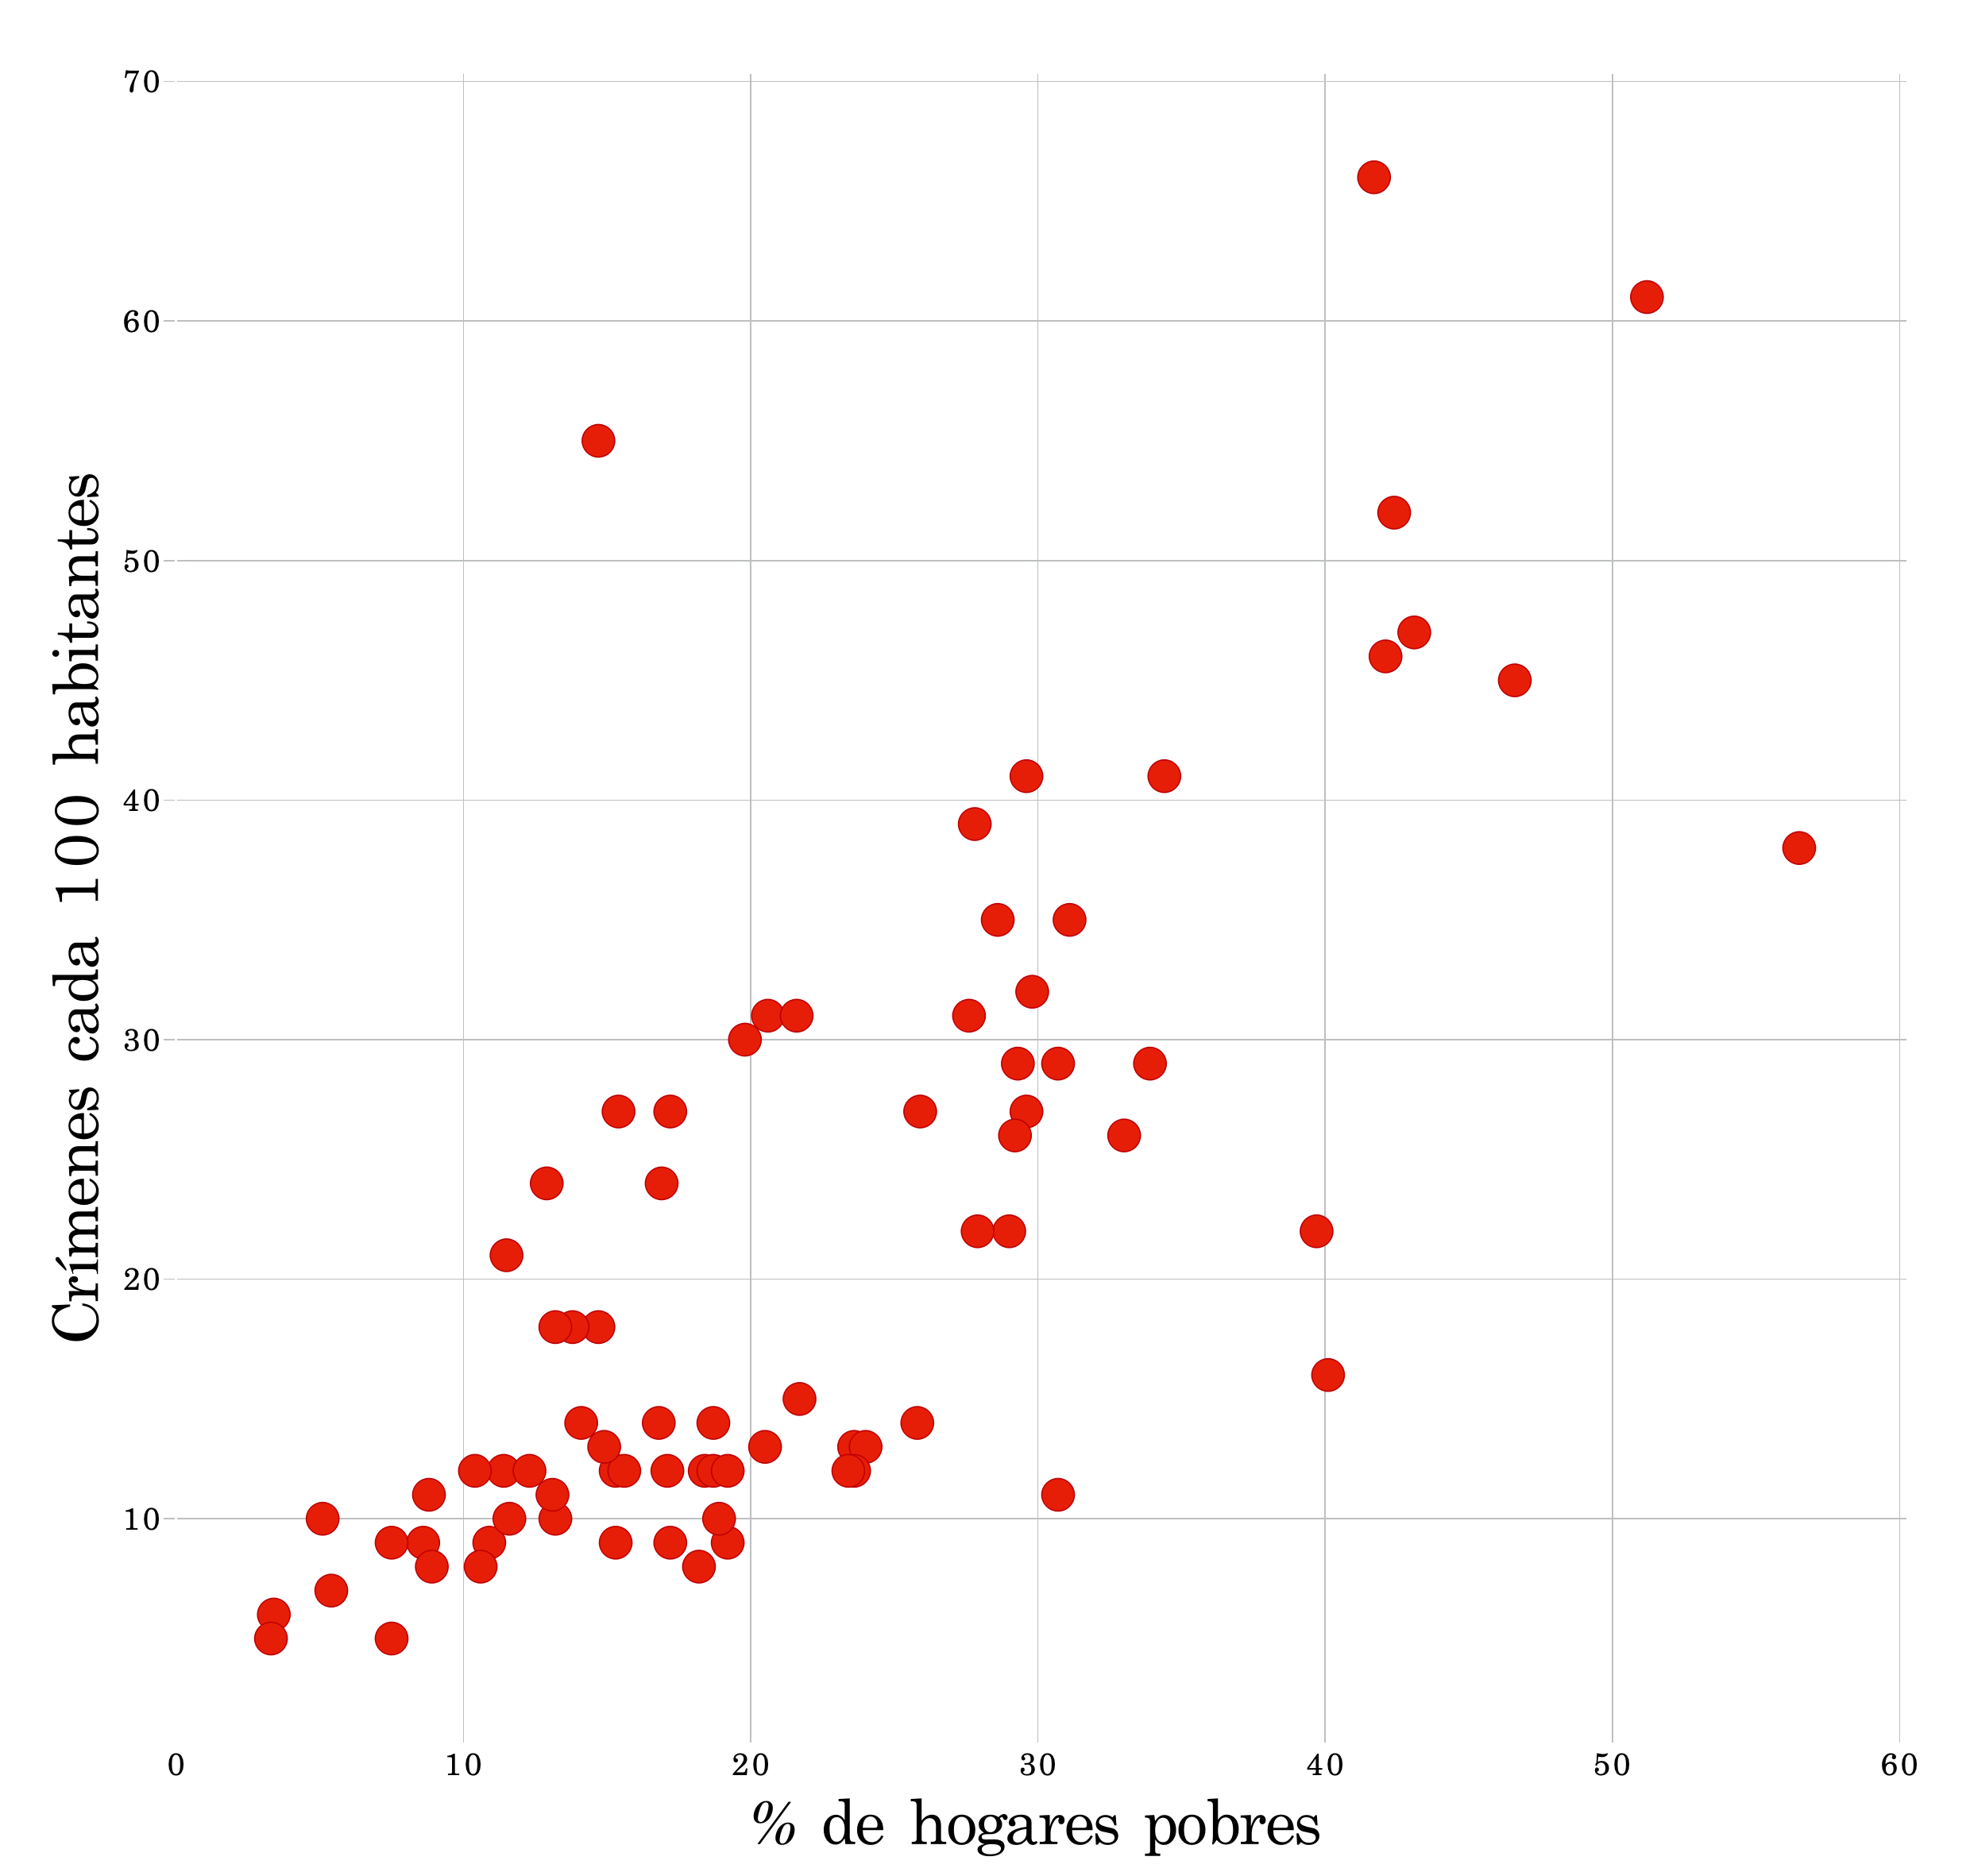
\includegraphics[scale=0.4]{Airbnb/Gráficos/grafico 1b airbnb.png}
    \source{Chicago Data Portal.}
    \label{fig:pob_cri}
\end{figure}

%describir qué tipo de mapa es, por qué eligieron hacer ese mapa/gráfico y qué muestra.
\textbf{Gráfico 2} El siguiente histograma muestra las tasas de respuesta de los \textit{hosts} de Airbnb en Chicago. En general, se observa que tienen tasas de respuesta muy altas (mayores a 70\%) y, particularmente, que la mayoría de los hosts tiene una tasa de respuesta entre 95\% y 100\%.

\begin{figure}[H]
    \centering
    \caption{Tasa de respuesta de anfitriones en Airbnb}
    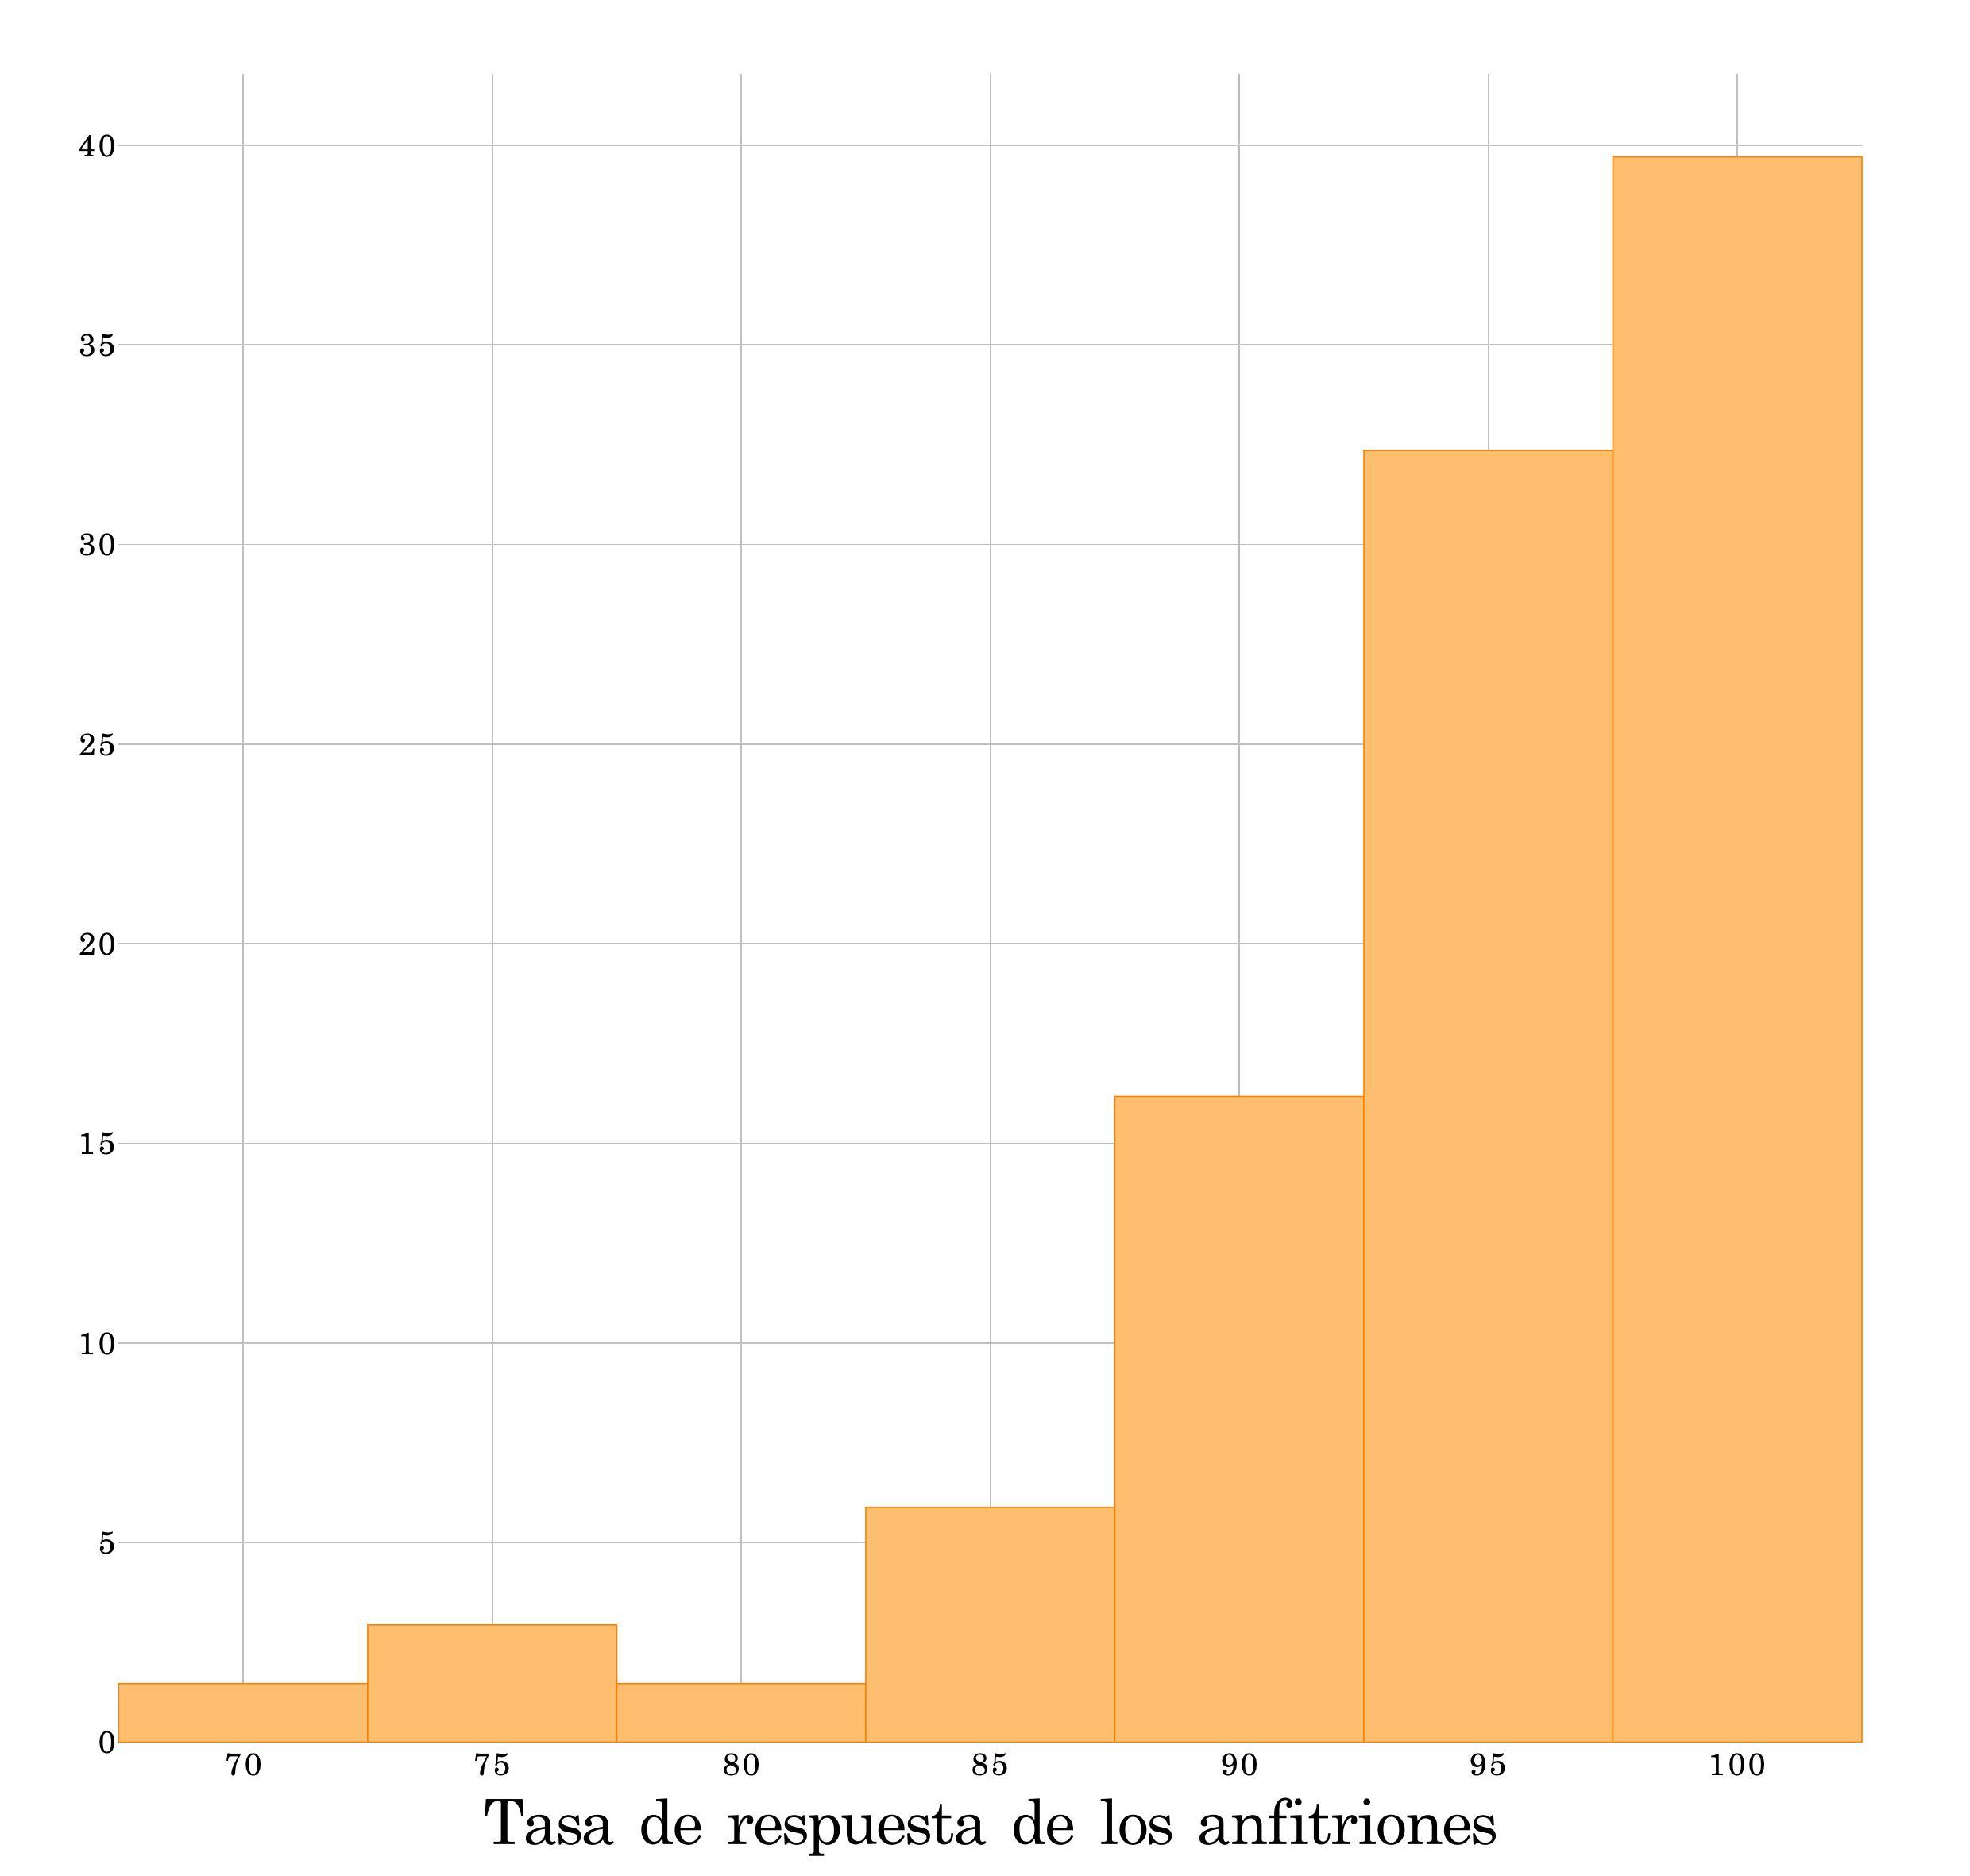
\includegraphics[scale=0.4]{Airbnb/Gráficos/grafico 2 airbnb.png}
    \source{Inside Airbnb.}
    \label{fig:response}
\end{figure}

\newpage
\textbf{Gráfico 3} En el siguiente gráfico, se observa cuál es la calificación promedio de los anfitriones por \textit{community} en Chicago. 

\begin{figure}[H]
    \centering
    \caption{Rating de hosts por \textit{community}}
    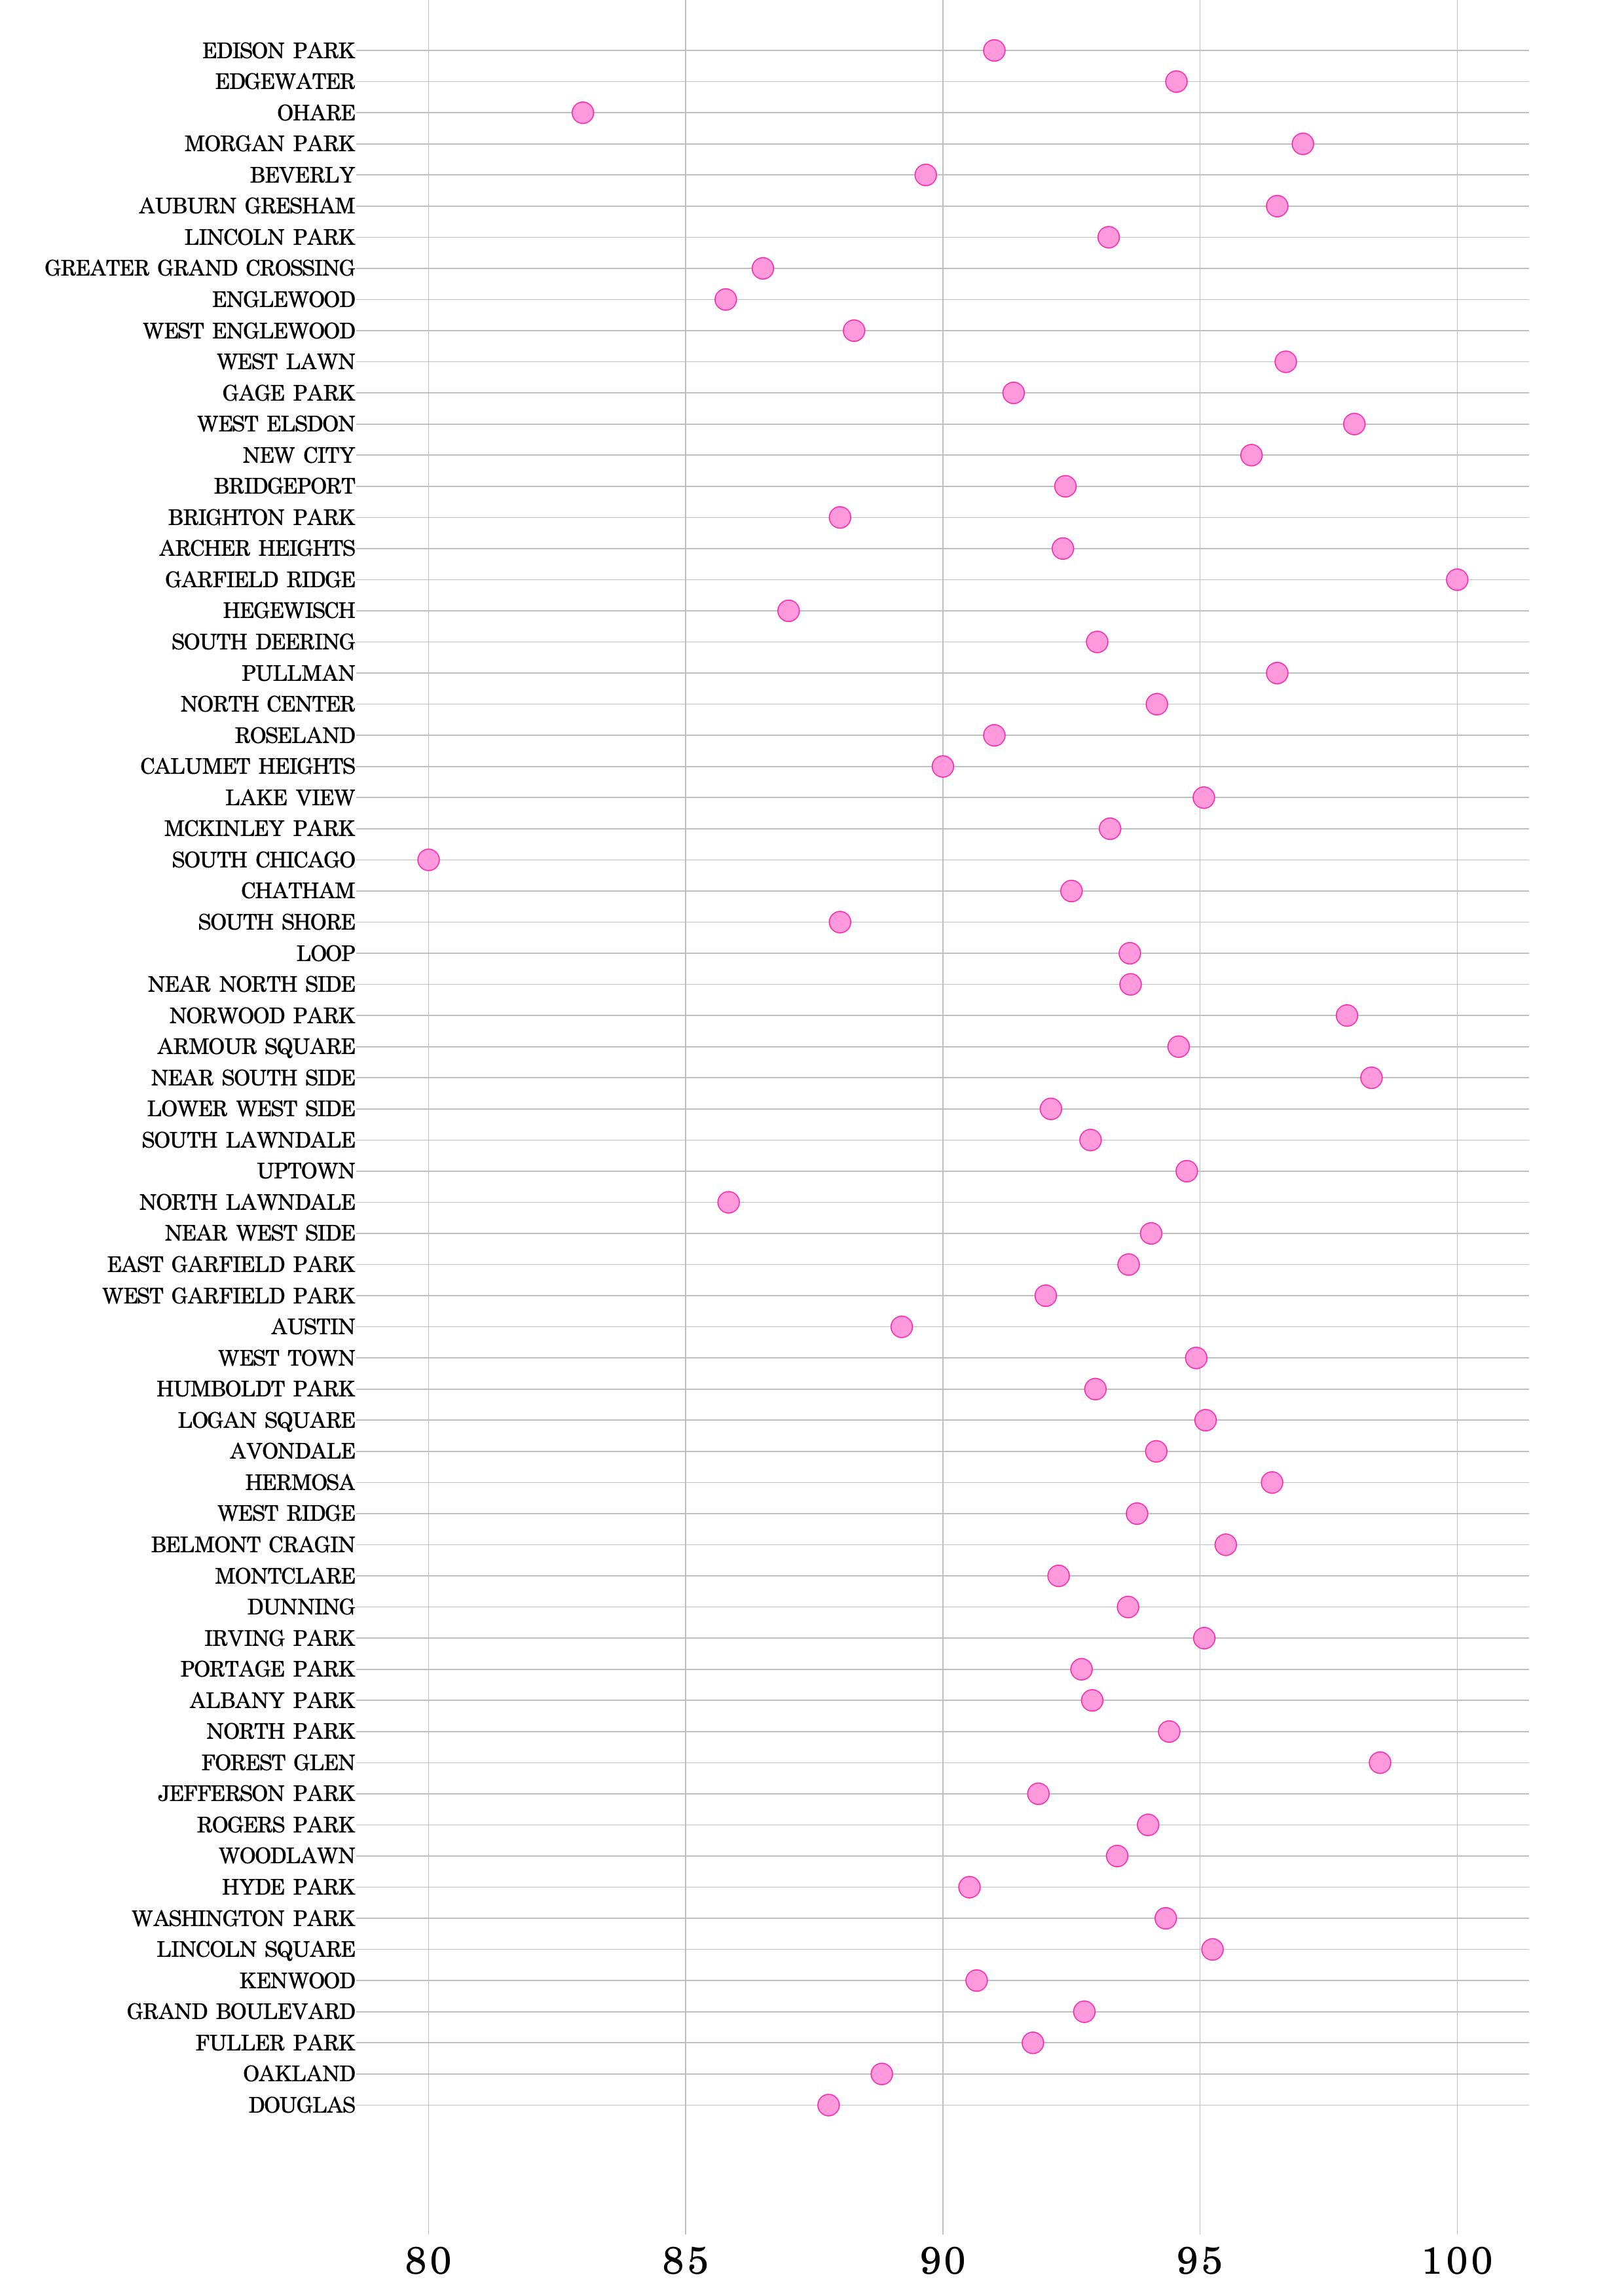
\includegraphics[scale=0.7]{Airbnb/Gráficos/grafico 3 airbnb.png}
    \source{Inside Airbnb}
    \label{fig:rating}
\end{figure}

\section*{Ejercicio 2: Buenos Aires} 


\textbf{Desempleo}
En los mapas presentados a continuación, se puede observar la tasa de desempleo en los diferentes municipios de la provincia de Buenos Aires. A partir de ellos, se observa que las tasas de desempleo más altas se encuentran en los municipios del sur de la provincia, en los partidos costeros y particularmente en el Área Metropolitana de Buenos Aires (AMBA), donde se concentran las tasas de desempleo más altas. Los demás municipios, excepto casos aislados, en promedio se encuentran en la franja de $1,47\%-2,87\%$.
\vspace{0.25cm}
\begin{figure}[H]
\caption{Tasa de desempleo}
\begin{subfigure}{.5\textwidth}
  \centering
  % include first image
  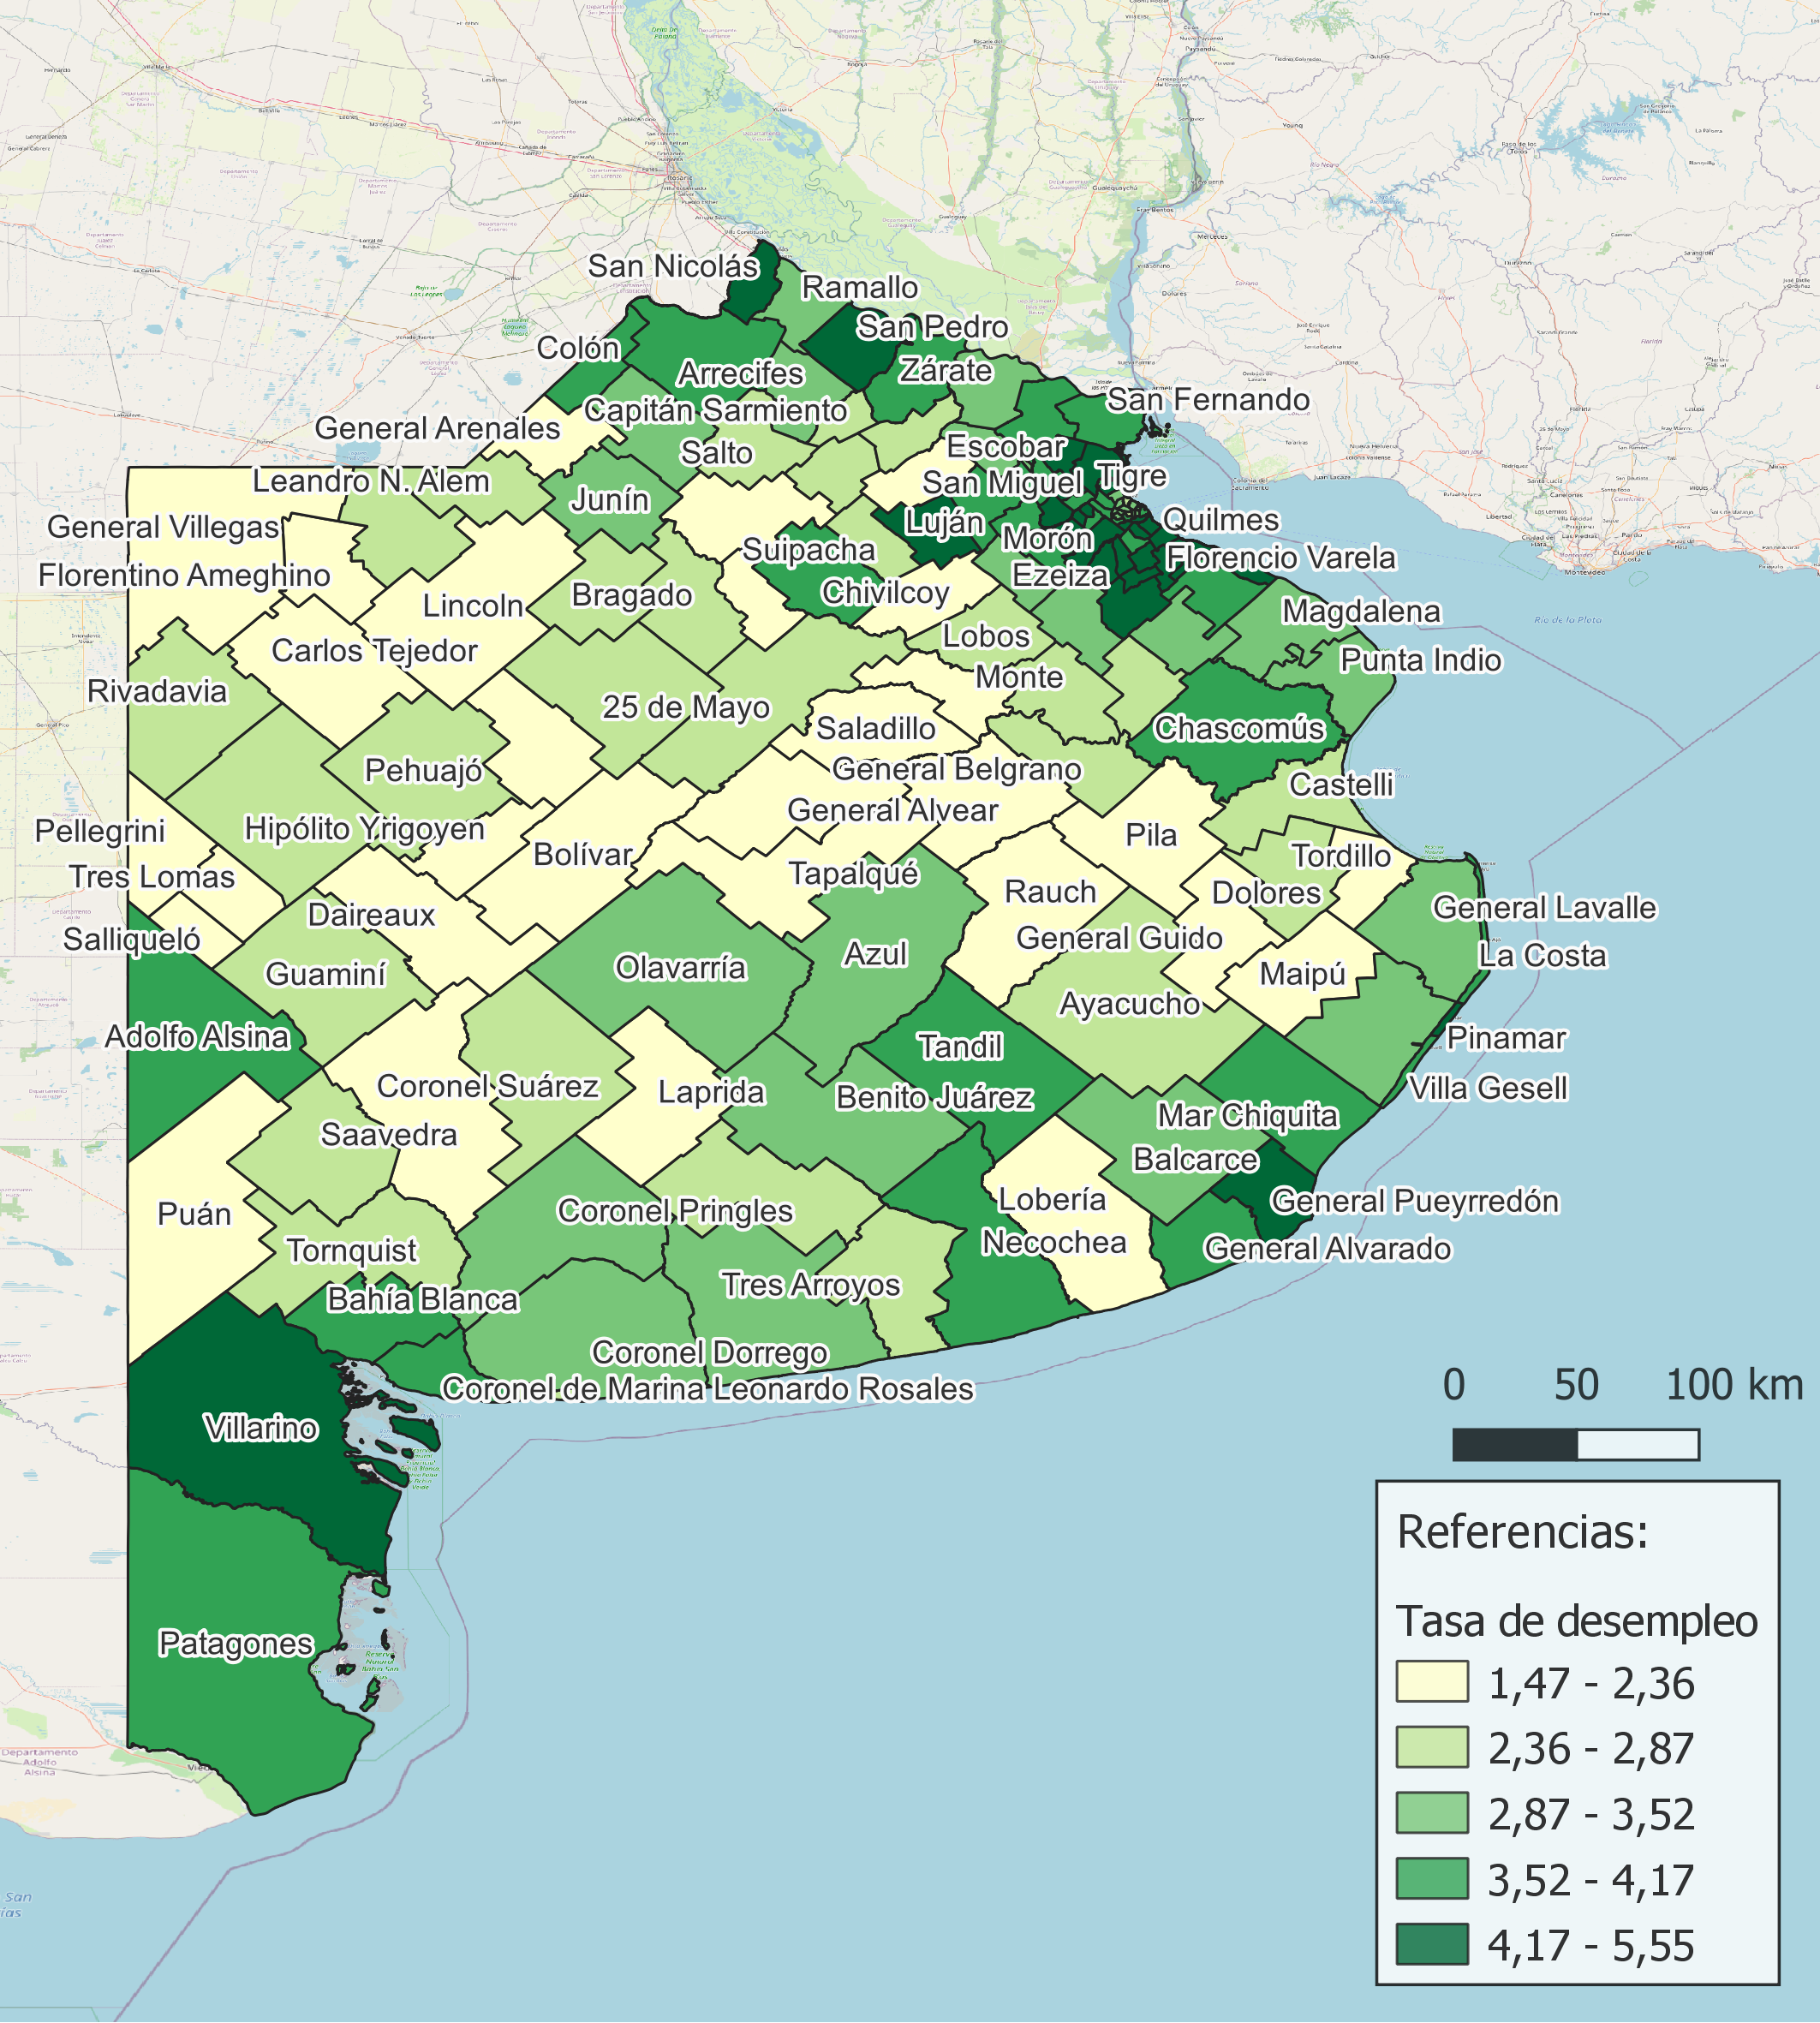
\includegraphics[width=.8\linewidth]{Buenos Aires/Gráficos/bsas1 Unemp.png}  
  \caption{Provincia de Buenos Aires}
  \label{fig:7a}
\end{subfigure}
\begin{subfigure}{.5\textwidth}
  \centering
  % include second image
  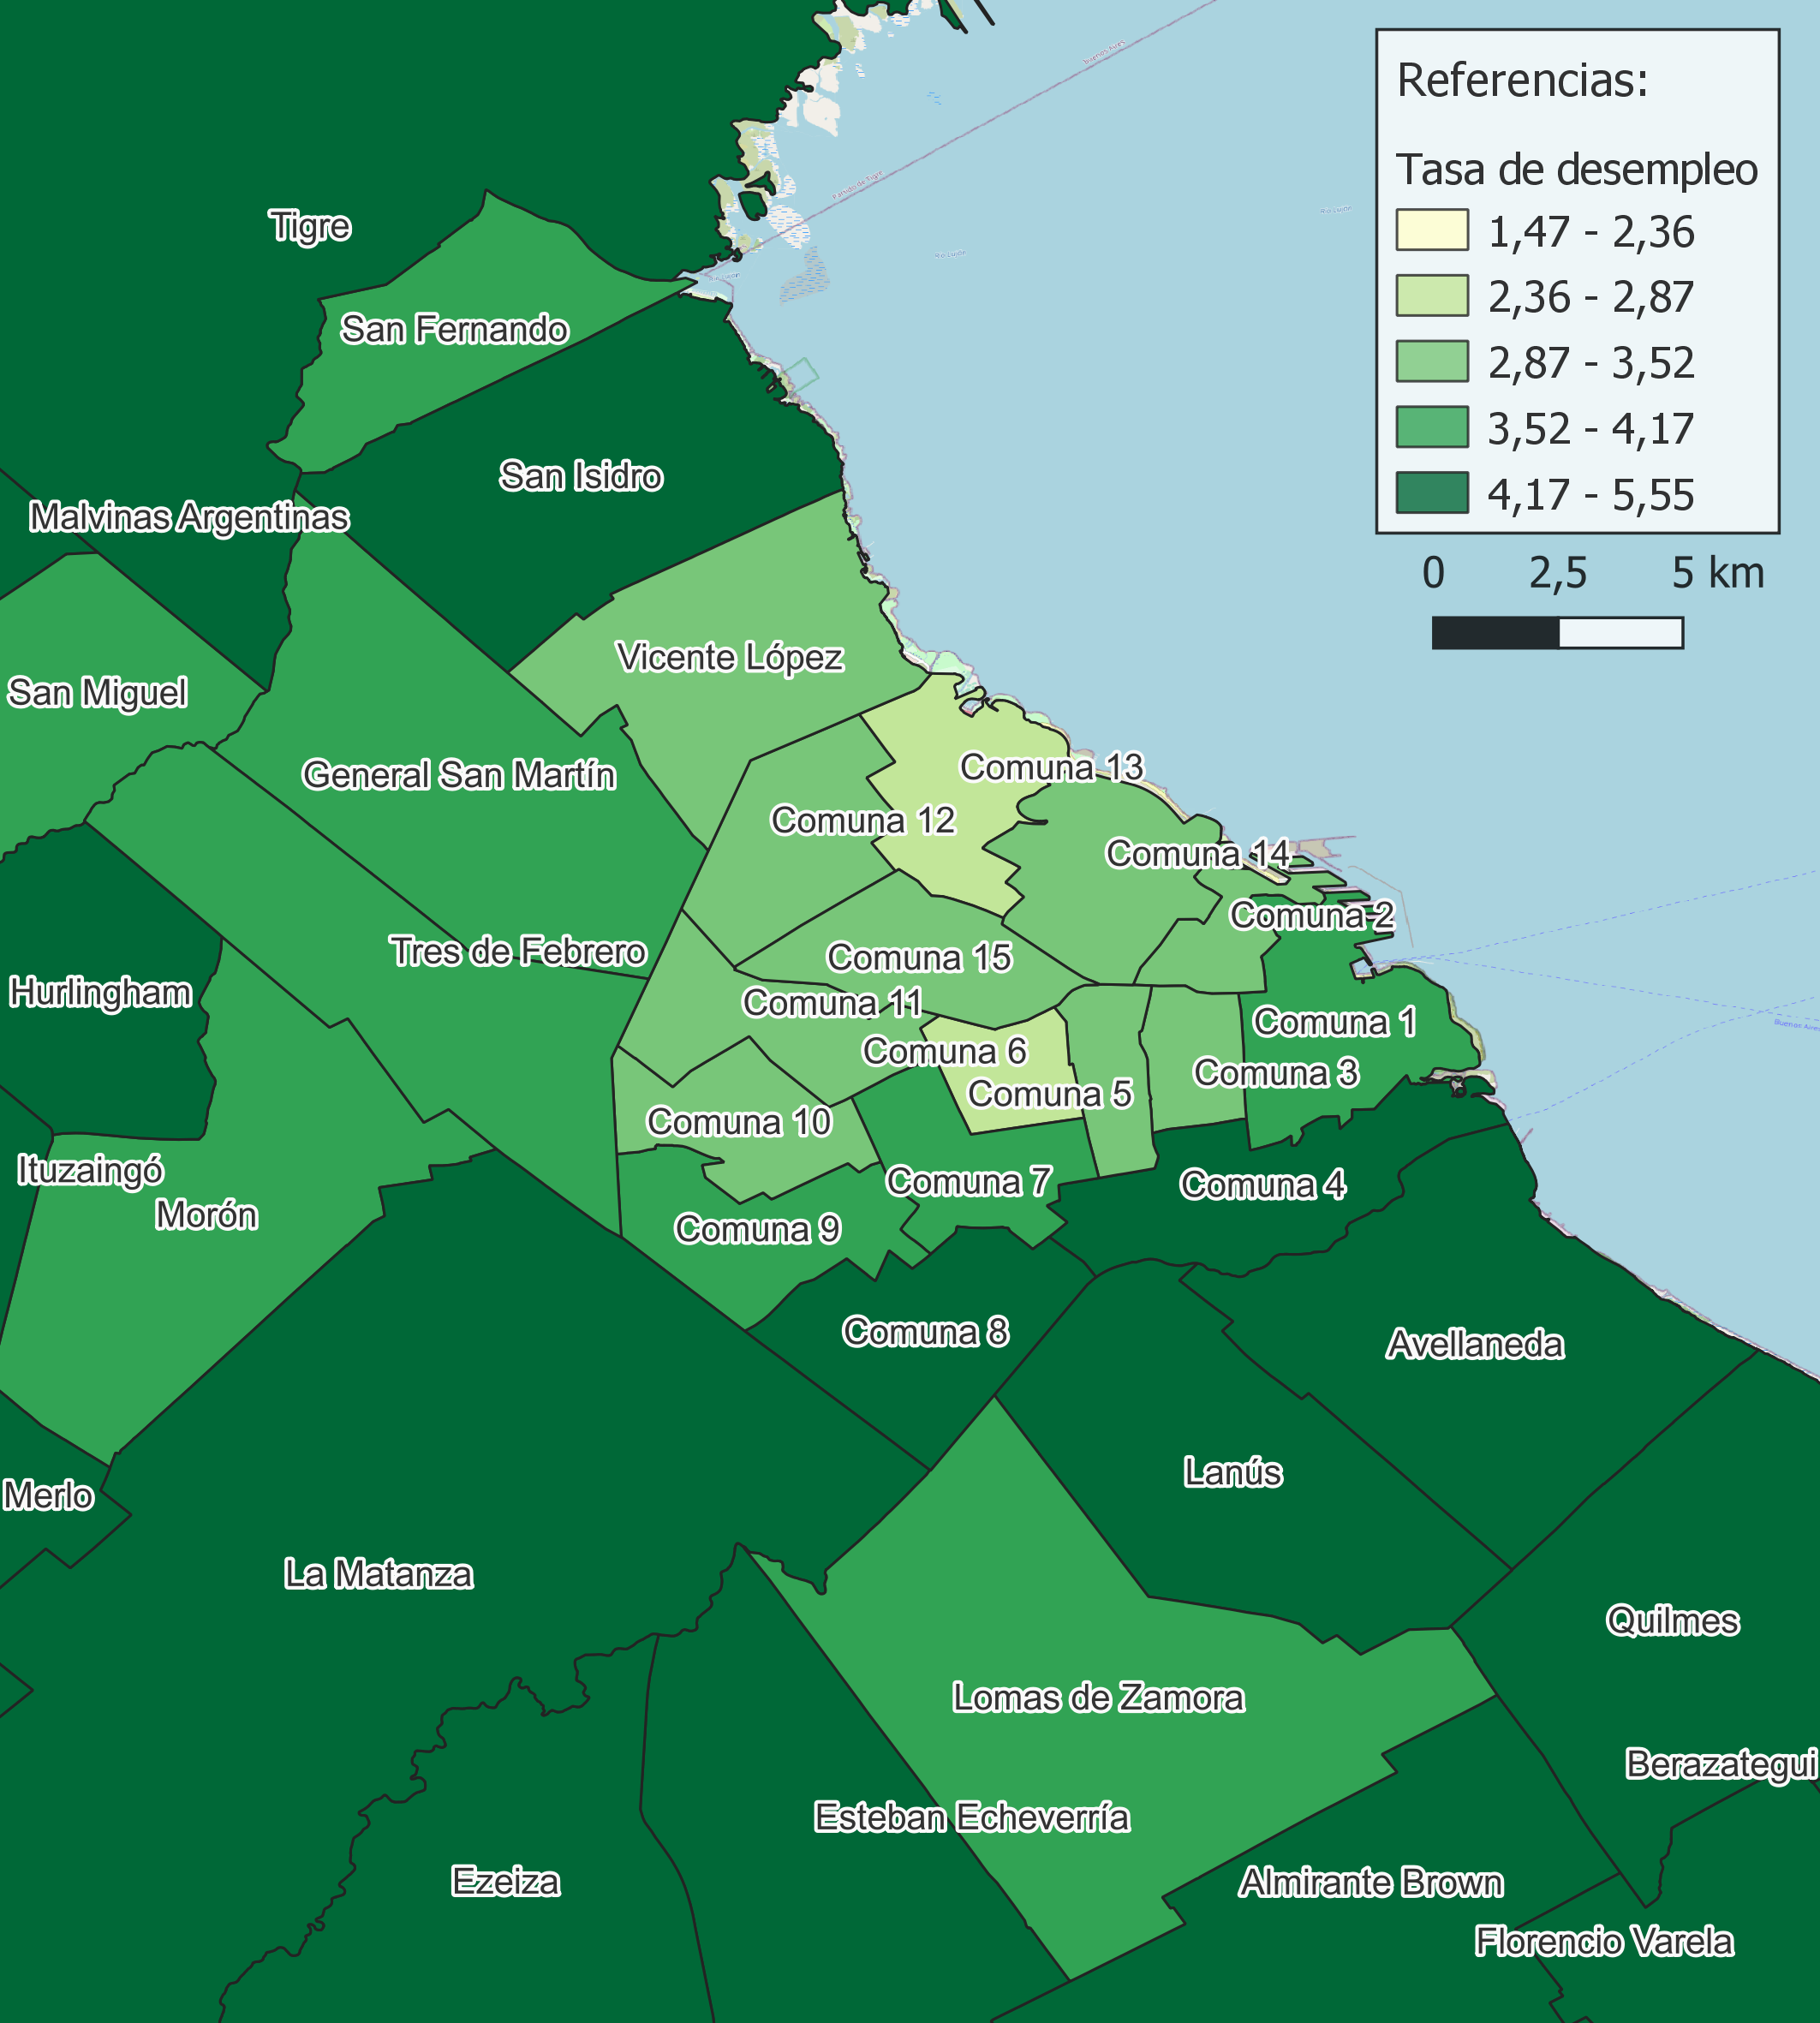
\includegraphics[width=.8\linewidth]{Buenos Aires/Gráficos/bsas2 Unemp.png}
  \caption{AMBA}
  \label{fig:7b}
\end{subfigure}
\label{fig:7}
\source{INDEC}
\end{figure}

\newpage
\textbf{Necesidades básicas insatisfechas} 
Por último, en los mapas presentados en la figura \ref{fig:8} a continuación, se muestra la tasa de necesidades básicas insatisfechas (NBI) por municipio en la provincia de Buenos Aires en el panel \ref{fig:8a} y particularmente en el AMBA en el panel \ref{fig:8b}. En línea con los mapas presentados anteriormente, se observa que los municipios del sur de la provincia y del AMBA son aquellos con tasas de NBI más altas. Sin embargo, es importante notar que los municipios / comunas pertenecientes a la Ciudad Autónoma de Buenos Aires y la zona norte de la provincia presentan las tasas de necesidades básicas insatisfechas más bajas del AMBA, a pesar de que los niveles de desempleo son, en general, altos en estos municipios. 

\begin{figure}[H]
\caption{Necesidades Básicas Insatisfechas}
\begin{subfigure}{.5\textwidth}
  \centering
  % include first image
  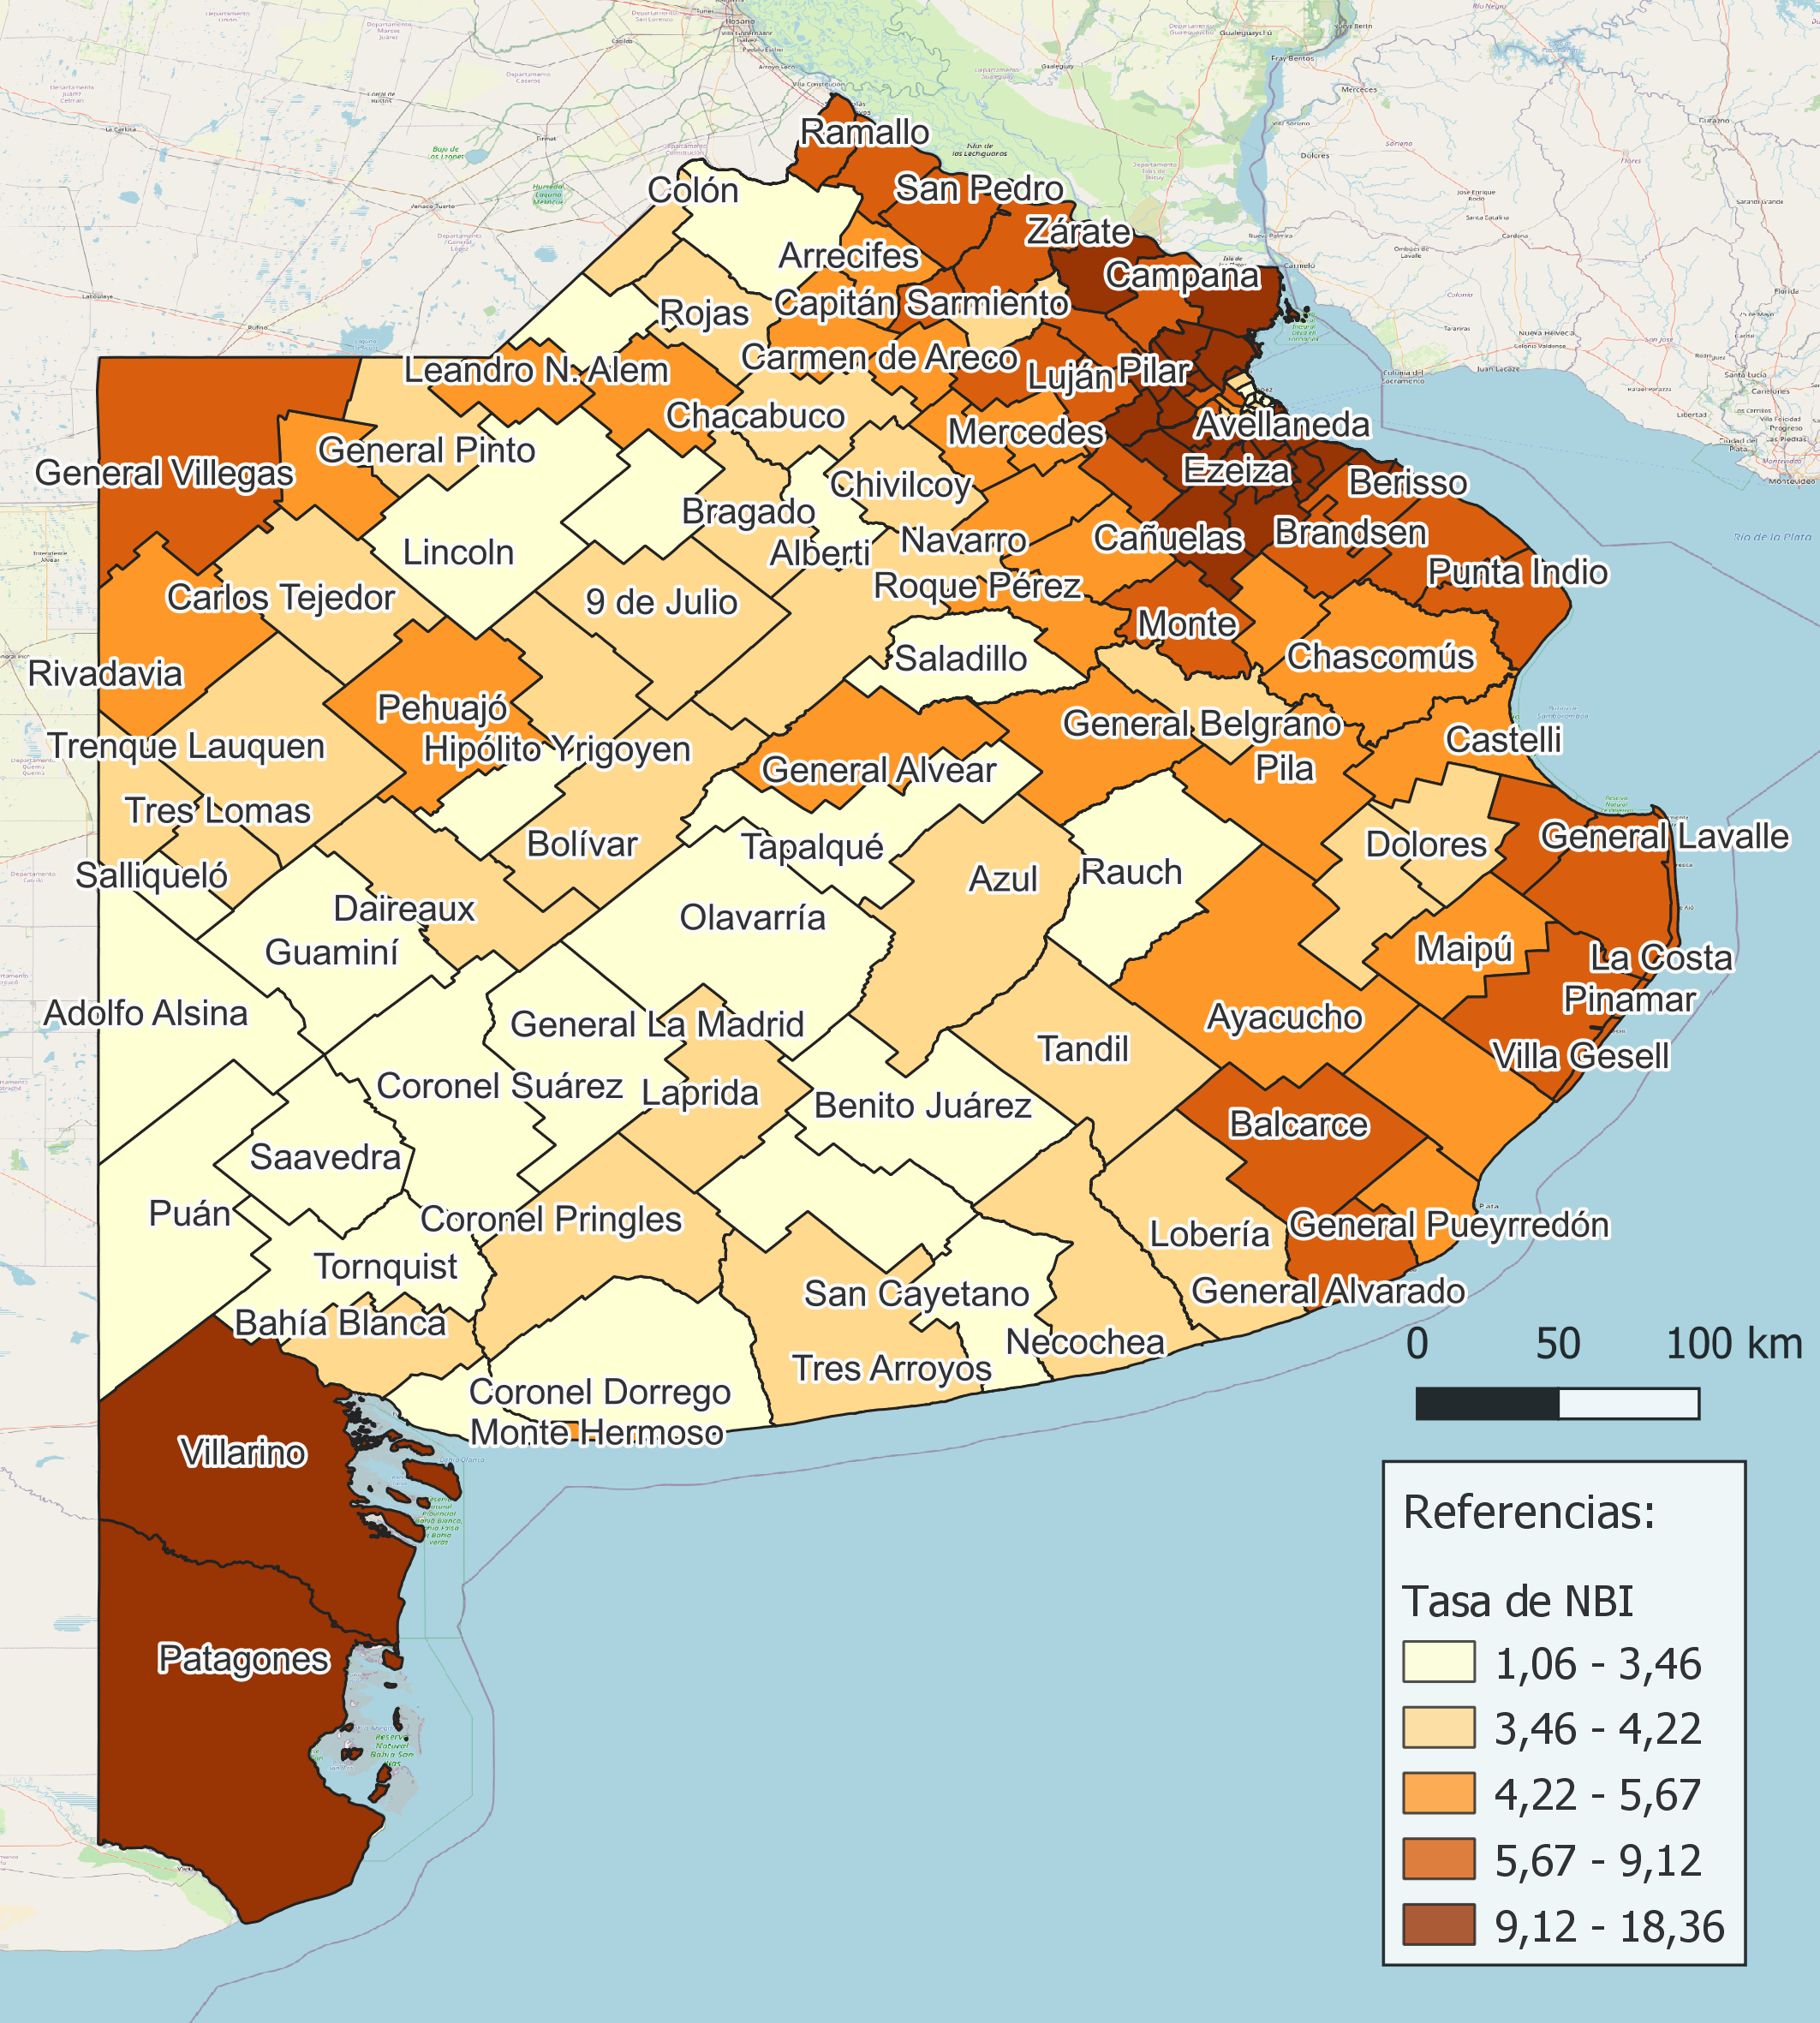
\includegraphics[width=.8\linewidth]{Buenos Aires/Gráficos/bsas4 NBI.png}  
  \caption{Provincia de Buenos Aires}
  \label{fig:8a}
\end{subfigure}
\begin{subfigure}{.5\textwidth}
  \centering
  % include second image
  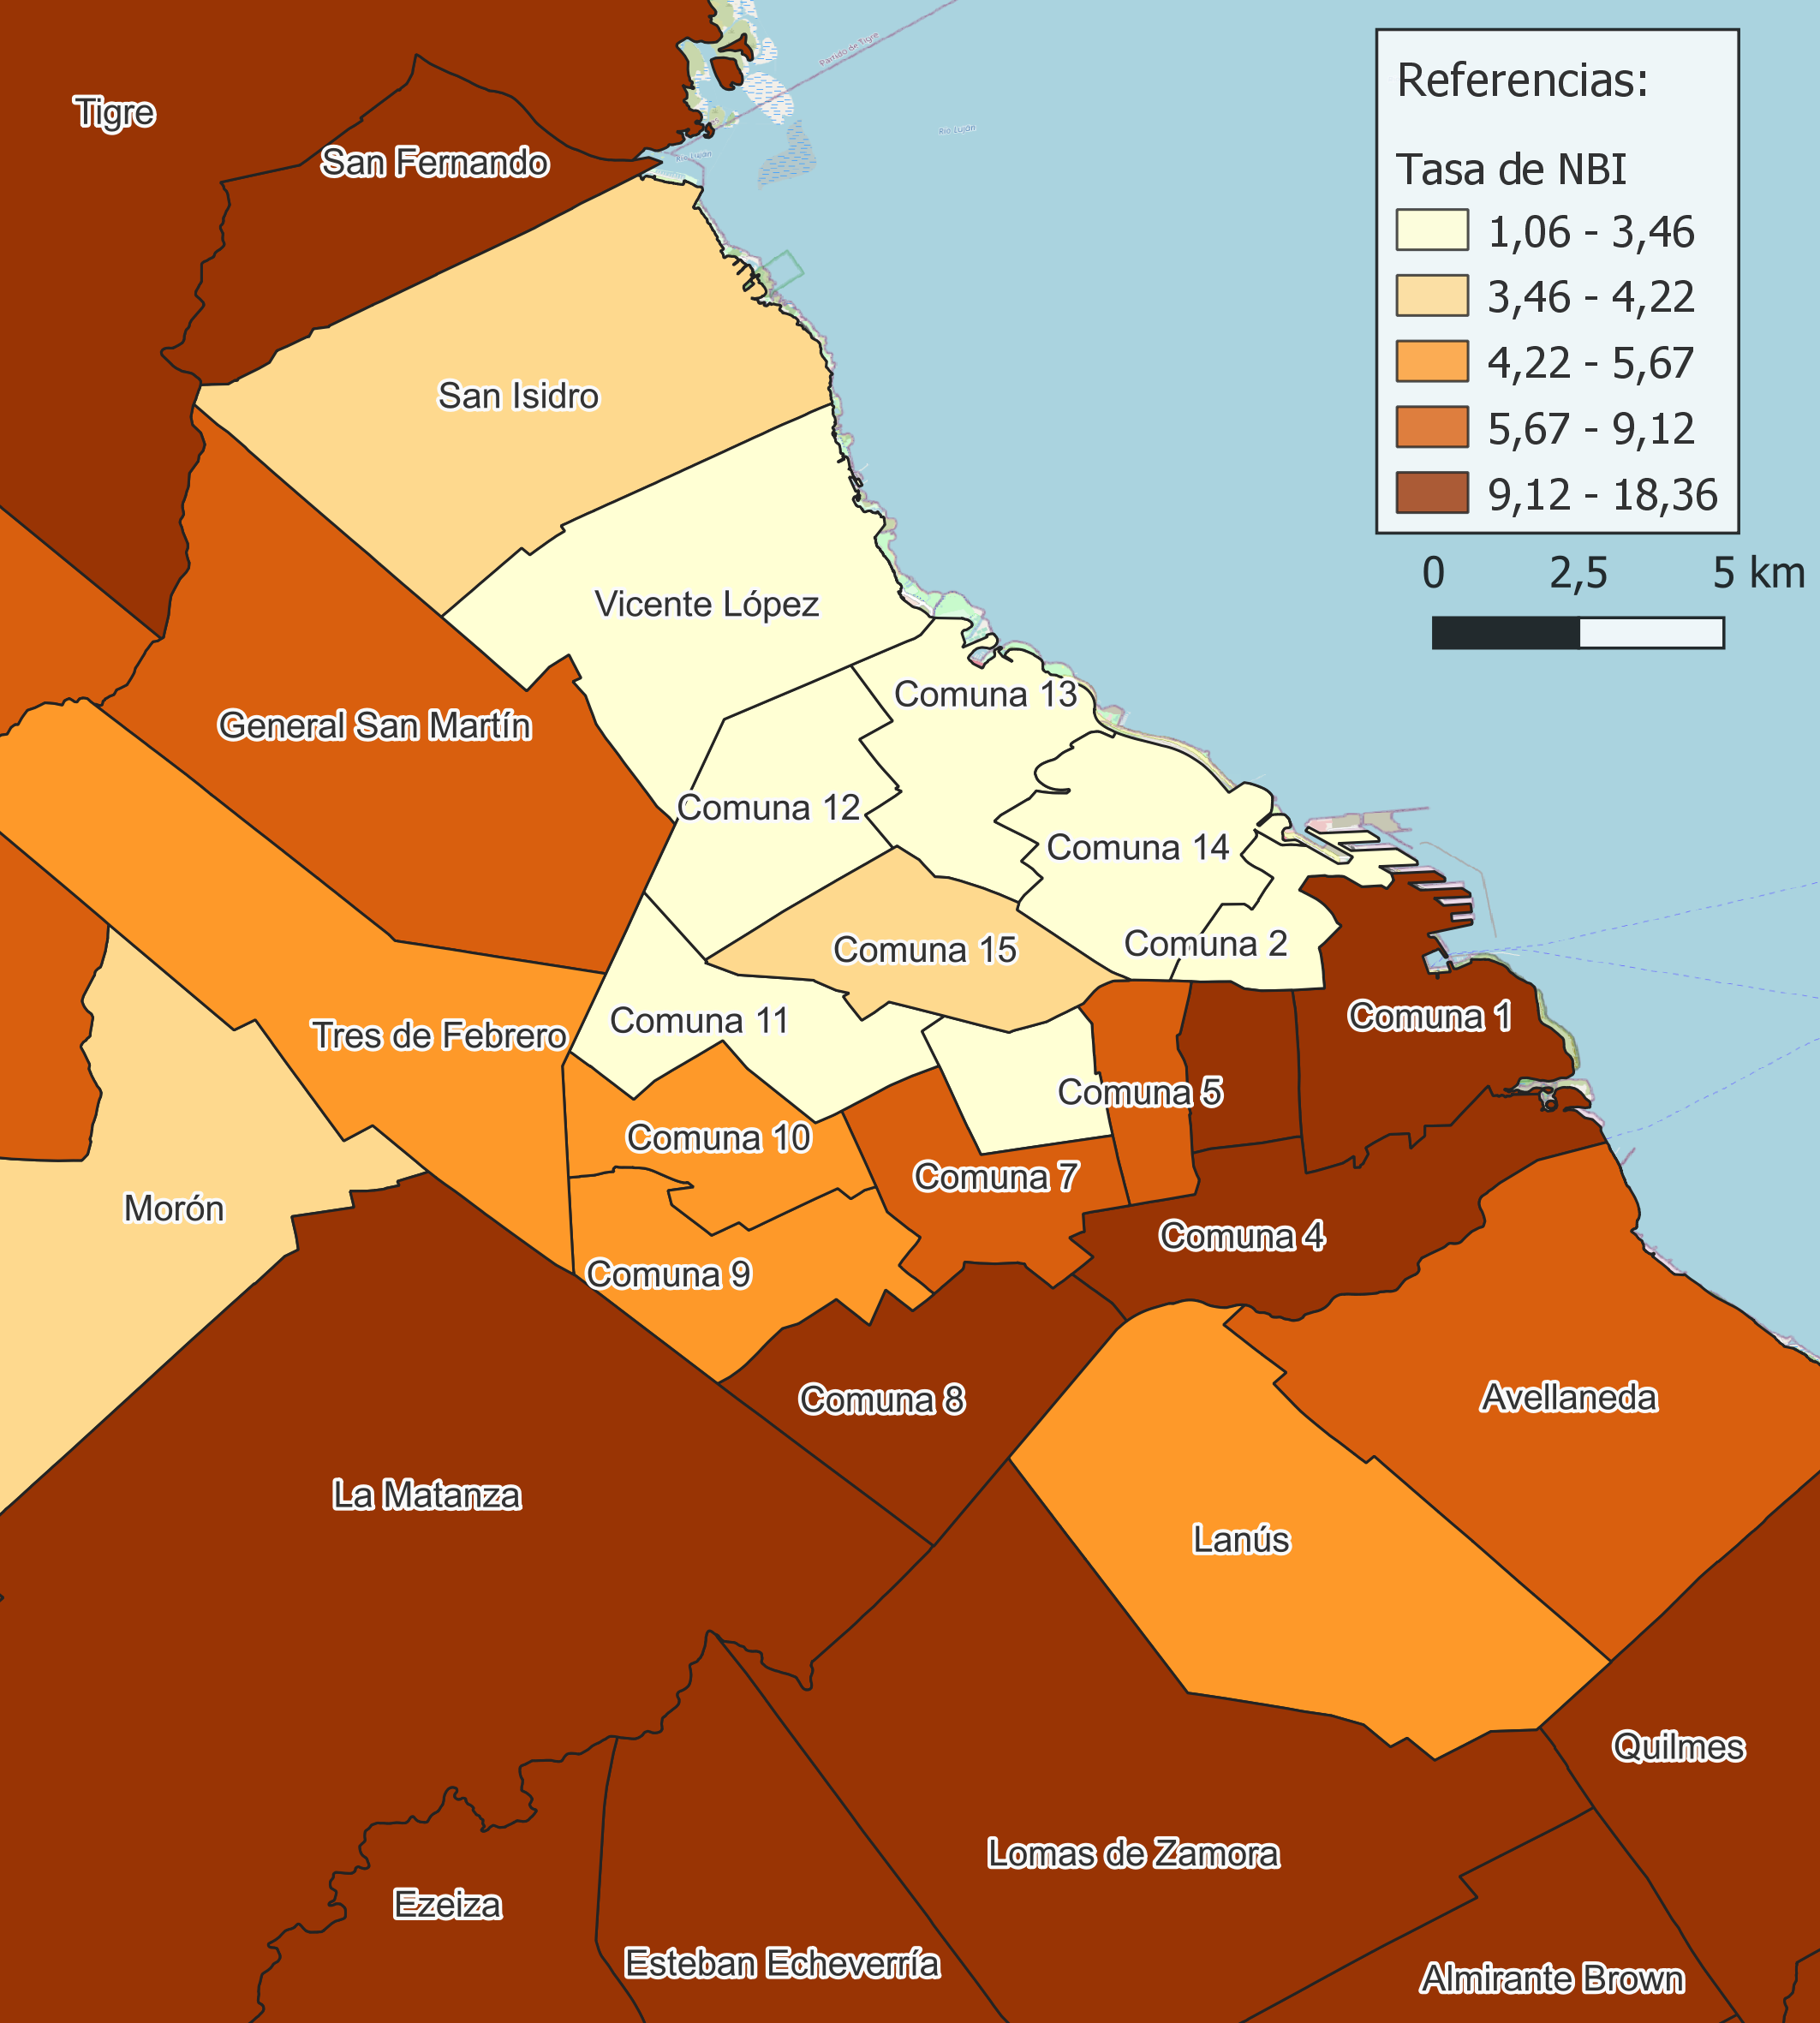
\includegraphics[width=.8\linewidth]{Buenos Aires/Gráficos/bsas3 NBI.png}
  \caption{AMBA}
  \label{fig:8b}
\end{subfigure}
\label{fig:8}
\source{INDEC}
\end{figure}

\end{document}
